\documentclass[a4paper, 12pt]{report}
\usepackage[english]{babel}
%\usepackage[T1]{fontenc}
\usepackage{graphicx}
\usepackage{float}
\usepackage{listings}
\usepackage[centertags]{amsmath}
\usepackage{amsfonts}
\usepackage{amssymb}
\usepackage{amsmath}
\usepackage{amsthm}
\usepackage{newlfont}
\usepackage{fancyhdr}
\usepackage{tesisty}
\usepackage{hyperref}
\usepackage[utf8x]{inputenc}
\usepackage[toc,page]{appendix}
\usepackage[ruled,vlined]{algorithm2e}
\usepackage{algpseudocode}



\lstset{basicstyle=\small\sffamily,
  numbers=none,
  frame=tb,
  columns=fullflexible,
  showstringspaces=false,
  breaklines=true
}



%-------------------------------
% DEFINIZIONE DEGLI ENVIRONMENT
%-------------------------------

\newtheorem{obs}{Osservazione}[section]
\newenvironment{oss}
    {\begin{obs}\begin{normalfont}}
    {\hfill $\square \!\!\!\!\checkmark$ \end{normalfont}\end{obs}}

\newtheorem{pro}{Problema}[chapter]
\newenvironment{prob}
    {\begin{pro}\begin{normalfont}}
    {\hfill $\spadesuit$ \end{normalfont}\end{pro}}

\newtheorem{teor}{Teorema}[section]
\newenvironment{teorema}
    {\begin{teor}\textit }
    {\hfill  \end{teor}}

\newtheorem{defn}{Definizione}[section]
\newenvironment{de}
    {\begin{defn}\begin{normalfont}}
    {\hfill $\clubsuit$ \end{normalfont}\end{defn}}

%-----------------------------
% CONFIGURAZIONE DELLA PAGINA
%-----------------------------

\hfuzz2pt % Don't bother to report over-full boxes if over-edge is < 2pt

\numberwithin{equation}{section}
\renewcommand{\theequation}{\thesection.\arabic{equation}}

\setlength{\parindent}{0pt}


%--------------------------
% MODIFICARE DA QUI IN POI
%--------------------------

\begin{document}

\dedicate{Inserire la dedica}

\corso{INFORMATICA} \titoloRelazione{\textbf{Vimond Analytics Platform}} 
\relatore{Valeria Cardellini}
\anno{A.A 2012/2013}
 \autore{Luzzi Matteo Remo}
 \correlatore{Glenn Skare Pedersenn}



\baselineskip=25pt

\intestazione

%------------------------------------------------
% INTRODUZIONE E RINGRAZIAMENTI (NON MODIFICARE)
%------------------------------------------------

\fancypagestyle{plain}{
\fancyhead{}\renewcommand{\headrulewidth}{0pt} } \pagestyle{fancy}
\renewcommand{\chaptermark}[1]{\markboth{\small Cap. \thechapter \textit{ #1}} {} }
\renewcommand{\sectionmark}[1]{\markright{\small  \thesection \textit{ #1}} {} }
\voffset=-20pt                         % distanza tra il limite superiore del foglio e l'intestazione
\headsep=40pt                          % distanza  l'intestazione ed il testo del corpo
\hoffset=0pt                           % misura equivalente al margine sinistro
\textheight=620pt                      % altezza del corpo del testo
\textwidth=435pt                       % larghezza del corpo del testo
\footskip=40pt                         % distanza tra il testo del corpo ed il pie' di pagina
\fancyhead{}                           % cancella qualsiasi impostazione per l'intestazione
\fancyfoot{}                           % cancella qualsiasi impostazione per il pie' di pagina
\headwidth=435pt                       % larghezza del'intestazione e del pie' di pagina
\fancyhead[R]{\rightmark} \fancyfoot[L]{\leftmark}
\fancyfoot[R]{\thepage}
\renewcommand{\headrulewidth}{0.3pt}   % spessore della linea dell'intestazione
\renewcommand{\footrulewidth}{0.3pt}   % spessore della linea del pi�di pagina

\pagenumbering{Roman} \tableofcontents
\newpage

\pagenumbering{arabic}

\fancyhead[R]{Introduction} \fancyfoot[L]{Introduction}
\fancyfoot[R]{\thepage}

\chapter*{Acknowledgement}
\addcontentsline{toc}{chapter}{Acknowledgement}
Finally I'm here writing the last pages of my academic career, a period full of satisfactions and delusions that made me the person who I am now. It would have not been the same without the people who influenced me. \\
I would like to thank first of all my supervisor Valeria Cardellini from university of Rome "Tor Vergata" for following me in this final project and giving me useful suggestions. I worked on this theis project as an intern in Vimond Media Solution company, located in Bergen (Norway). A great thank to Glenn, Vegard and Kine for considering me as a suitable candidate for this research project, to Helge for being such a great presence, more like a father rather than a CEO and to anyone else who has helped me activetly or just spent time for a talk. I don't know if I could have had a better exerience anywhere else.\\
università, bergen, amici (friends from a lifetime), famiglia

bergen: Andrea A. Andrea C. Solvejg, Dario, Nicole, Daniele, Alessandra, Josie, Camille, Alix, Julia, Elvira, Roberto

amici: Alessandro, Andrea, Nicholas, Francesco, Marta, Manuel, Piergiorgio, Giuseppe

Finally, the big thank goes to my parents, Angelo and Gabriella. None of this could have ever been possible without their constant support. Thanks for being an inspiration in every desition I took.

\chapter*{Abstract}
\addcontentsline{toc}{chapter}{Abstract}

From early 2000s, when the term Big Data was first coined, the evolution of technology has imposed new challenges on the design of data systems. The growing amount of data highlighted the limits of traditional architectures, therefore research moved its focus on new solutions able to handle it. Big data are also a remunerative market. It has been measured that, in 2013, the vendors revenue derived by related hardware, software and services was more than 18 million dollars, with a 58\% boost respect to the previous year \cite{bib29}. It is estimated that by 2017 the revenue will be more than 50 million dollars. Recently, we could notice an evolution for cloud-based big data services for large-scale analytics. More and more companies realized about the benefits of data analysis in order to carve out advantages in the market. A survey of 2013 \cite{bib32} shows that more than 50\% of the survey respondents declared that investing on analytics improved organization's competitive position, in terms of identifying new ways to perform sales and understanding users behavior for targeting them with ad-hoc campaigns.\\
Traditionally, for processing a high volume of data, a batch approach with tools like Hadoop is used, specially after the release of Yarn \cite{bib24}, which has broadened its applicability domains. However, some use cases, require to process data in nearly real-time, in order to have the possibility of taking business decisions quickly according to their results. What normally happens, is that these two ways of processing data are independent and are implemented in two different systems.\\
In response to a need of new approaches and patterns for big data processing, this thesis proposes a new architectural pattern: ``VimondAnalytics", named after the company (Vimond Media Solutions \cite{bib1}) where this master thesis project was carried out. It is based on the Lambda architecture, a pattern proposed by N. Marz \cite{bib2}, which provides a new way to combine the classic batch and real-time computations in one solution. Data are analyzed in two layers in parallel, batch and real-time respectively, and their results are stored on dedicated databases and finally merged in the serving layer. High latency of batch results is compensated by the real-time layer. This gives high availability to the system at the cost of eventual consistency according to the CAP theorem \cite{bib33}. Even though Lambda architecture was first introduced in 2011, it has not been deeply investigated up to now, and we could find in literature only few examples of complete implementations \cite{bib30}, \cite{bib31}. The purpose of this thesis is to provide a proof of concept implementation, and show its applicability in the fields of big data analytics. We will show how the initial pattern of Marz can be simplified, by eliminating intermediate databases, performing all the data aggregation and merging directly into the serving layer. The developed system has been deployed on AWS\footnote{https://aws.amazon.com} (Amazon Web Service). \\
The results obtained are straightforward: having a safe data deletion mechanism leads to a decrease in the required time to query the system, compared to a classic solution where all data are ingested into the serving layer and never deleted. In case of throttled input frequency, we will show that VimondAnalytics query time is limited by an upper and a lower bound, depending on the chosen batch time window. We will also show how the system reacts to some failures of single components of the system. However, some of the results, are tightly coupled with the frameworks used for the implementation, and might not be valid outside this context.\\
The rest of this report is structured as follows:
\begin{itemize}
\item Chapter 1 gives an introduction of the context of this work, specifically about big data analytics and what is the state of the art in term of architectures and patterns for handling them. 
\item Chapter 2 briefly analyzes what are the tools and technologies used in this work, highlighting their main features and their architectures.
\item Chapeter 3 describes VimondAnalytics architecture in detail. Great attention is given to each different layer and it is explained how they all cooperate in order to have a working solution.
\item Chapter 4 discusses a possible implementation of VimondAnalytics using the tools introduced in chapter 2.
\item Chapter 5 shows the results obtained with the proposed framework. General purpose tests were run in order to validate these results. For completion, the system was also tested under some common failover scenarios.
\item Finally, chapter 6, summaries the work carried out in this thesis project. Furthermore, it outlines some future work scenarios in terms of enhancement of the current system features and applicability domains. 
\end{itemize}
\vspace{\fill}
\textbf{Keywords:}
Big data, analytics, Lambda architecture, batch processing, real-time processing, cloud computing, distributed systems

\fancyhf{} %elimina header/footer vecchi

\fancyhead[R]{Chapter \thechapter} \fancyhead[L]{\leftmark}
\fancyfoot[R]{\thepage}





%---------------------
% INCLUSIONE CAPITOLI
%---------------------

\chapter{Theory}
\label{chap:chaper1}

\section{BigData}

\section{Analytics}

\subsection{Existing solutions}

\section{BigData architectures}
\chapter{Big Data tools}
\label{chap:chapter2}
In this chapter we will describe the tools used for implementing a working prototype based on Lambda architecture paradigm previously explained. The scope of this thesis is not to make a survey of modern technologies for big data and here we will give just an overview highlighting purpose and main features of each used tool. For a better understanding of these tools, the reader is invited to consult additional resources about them.
\section{Kafka}
Apache Kafka \cite{bib19} is a general purpose distributed publish-subscribe message system originally developed at Linkedin and then opensourced in 2011 and inserted in the Apache ecosystem. The architecture is composed by one or more servers, also known as \textit{brokers}, which rely on Apache Zookeeper for coordination.\\
The key abstraction in Kafka is a topic: \textit{producers} publish messages to a topic and \textit{consumers} subscribe to one or more topics. A single topic is composed by a set of partitions, distributed and replicated among all the brokers in the cluster. For each partition there is a master replica and a set of slaves. Since normally there are more partitions than brokers, a broker can play the role of master some partitions and the role of slave for others. For each partition are saved metadata about consumers positions, also called offsets. An offset represents a checkpoint for that consumer, messages before it are assumed to be correctly processed and the next time a consumer makes a fetch request, the broker will forward messages starting from the last offset. The consumer, anyway, is still able to reprocess already committed messages, for instance in response to a failover event.\\
\begin{figure}[h]
        \centering
        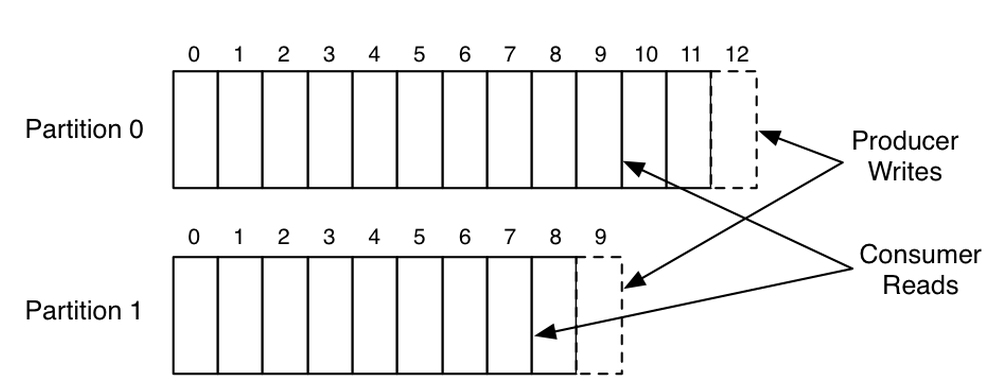
\includegraphics[width=12cm]{imgs/kafka-topic}
\caption[Kafka topic]{A 2-partitions topic with one producer and one consumer.\protect\footnotemark}
        \label{kafka-1}
\end{figure}
\footnotetext{https://engineering.linkedin.com/kafka/benchmarking-apache-kafka-2-million-writes-second-three-cheap-machines}

What it is interesting in Kafka is how messages are forwarded from the producer to the consumer through the brokers. Unlike other messaging systems which process  messages in-memory, Kafka does a strong usage of the filesystem: messages are immediately stored on filesystem and not deleted when read by a consumer but retained according to a configurable period. This avoid any kind of data loss for every committed message, even in case of brokers failure. The only information retained by brokers is the consumers positions across the topics. These information are generally stored on Zookeeper. \\
Kafka allows to implement either a \textit{queuing} or a \textit{publish-subscribe} logic introducing the abstraction of \textbf{consumer group}.
Each consumer labels itself with a  group name and is it responsible for reading from one or more partitions of a topic. Kafka ensures than no more than one consumer per group reads from a partition: if in the group there are more consumers than partitions, some of them will stay idle. In the opposite scenario, a consumer will read from more than one partition.
If all the consumers belong to the same group, then the system works as a queue, balancing the load across the consumer group. If all the consumers have different groups, then the system works as a standard publish-subscribe.\\
\begin{figure}[h]
        \centering
        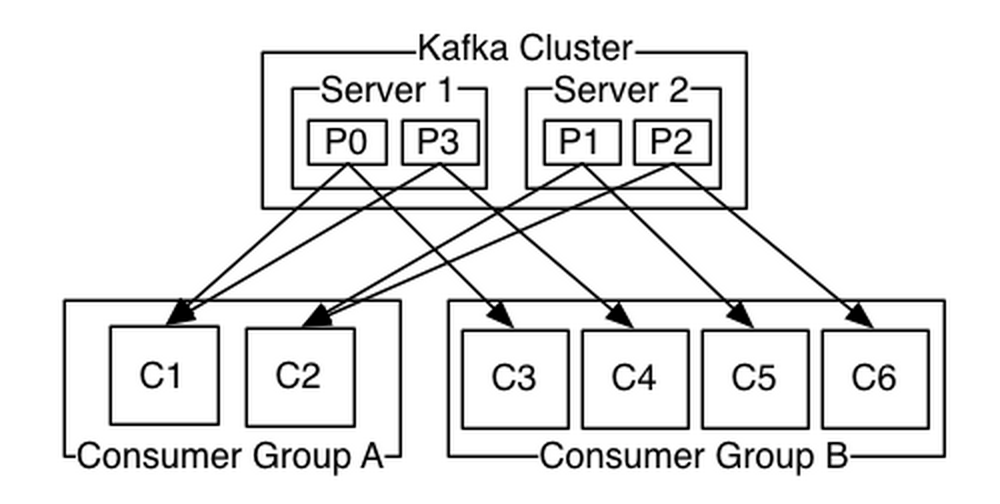
\includegraphics[width=12cm]{imgs/kafka-cgroup}
\caption[Kafka consumer group]{Two consumer groups read from a 4-partition topic.\protect\footnotemark}
        \label{kafka-2}
\end{figure}
\footnotetext{http://kafka.apache.org/documentation.html}

Having the concept of the consumer group implies a total order over the messages within each partition: the order on how are messages are read inside a partition is the same for every consumer who subscribed that partition.\\
As a conclusion, is worthy mention that Kafka implements by default a \textit{at-least-once} message semantic in the following way:
\begin{itemize}
\item Producer: when publishing a message and having a network error, the producer can't be sure if the message has been correctly committed to the broker.
\item Consumer: a message is said to be fully processed (from a broker perspective) only when its offset has been committed. The best the consumer can do is, read the message, process it and then commit the offset. If the consumer crashes  before committing the offset but after processing the message, the one taking over will process the same message.
\end{itemize}

\section{Hadoop}
\label{yarn}
Hadoop is an open-source suite for scalable fault-tolerant distributed computing written in Java. Based on Google's  \textit{Map-Reduce} \cite{bib25} approach, it was first developed in order to run MapReduce jobs for processing a web crawl. The rapid increase of popularity led to an abuse of the original computing paradigm exposed by Hadoop such as run heterogeneous task in a multi-tenant environment. In 2013, a second version of Hadoop, YARN \cite{bib24}, was released with the purpose of compensate the limitations of Hadoop first version, in primis decouple the programming model from the resource management layer and support a multi-tenancy job scheduler. 
\begin{figure}[h]
        \centering
        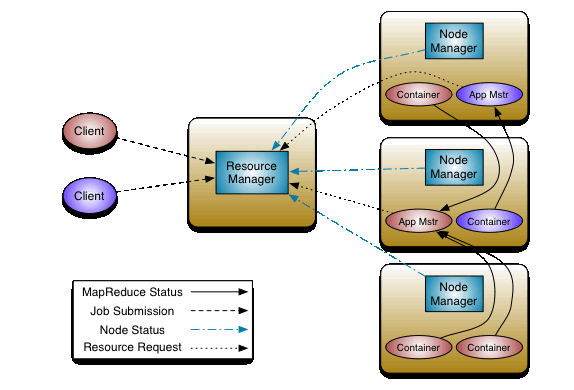
\includegraphics[width=12cm]{imgs/yarn-architecture}
\caption[YARN architecture]{YARN architecture\protect\footnotemark}
        \label{yarn-1}
\end{figure}
\footnotetext{http://hadoop.apache.org/docs/r2.7.0/hadoop-yarn/hadoop-yarn-site/YARN.html}
The architecture of YARN is composed by a global per-cluster \textit{Resource Manager (RM)} with duties of scheduling jobs submitted by clients and allocating resources when needed by the applications running on the cluster. Having a centralized coordinator enables scheduling properties of fairness, capacity and locality. The architecture is completed by one or more \textit{Node Managers (NM)} running on each slave node in the cluster. NMs are the workers daemons, in charge of monitoring the execution of the applications running on its node. Resources are spawned across running applications in form of \textit{containers}. A per-application daemon called \textit{Application Master (AM)} dynamically requests to the RM bundles of resources (containers) in order to execute the application it is responsible of. In this scenario, the RM is agnostic of the applications logics as it only replies to resources requests. MapReduce is now only a class of applications Hadoop YARN supports and several computation framework implementing different programming models has been adapted for being executed on top of YARN (Spark, Storm, Tez, Giraph and others).

\subsection{HDFS}
Hadoop distributed storage implementation is called HDFS (Hadoop Distributed File System). It is a highly efficient storage solution perfectly integrated with applications running on Hadoop, supporting the main operations of a normal filesystem and structured in a folder hierarchy. It is composed by a master/slave architecture with by one \textit{Namenode} and at least one \textit{Datanode}.
\begin{figure}[h]
        \centering
        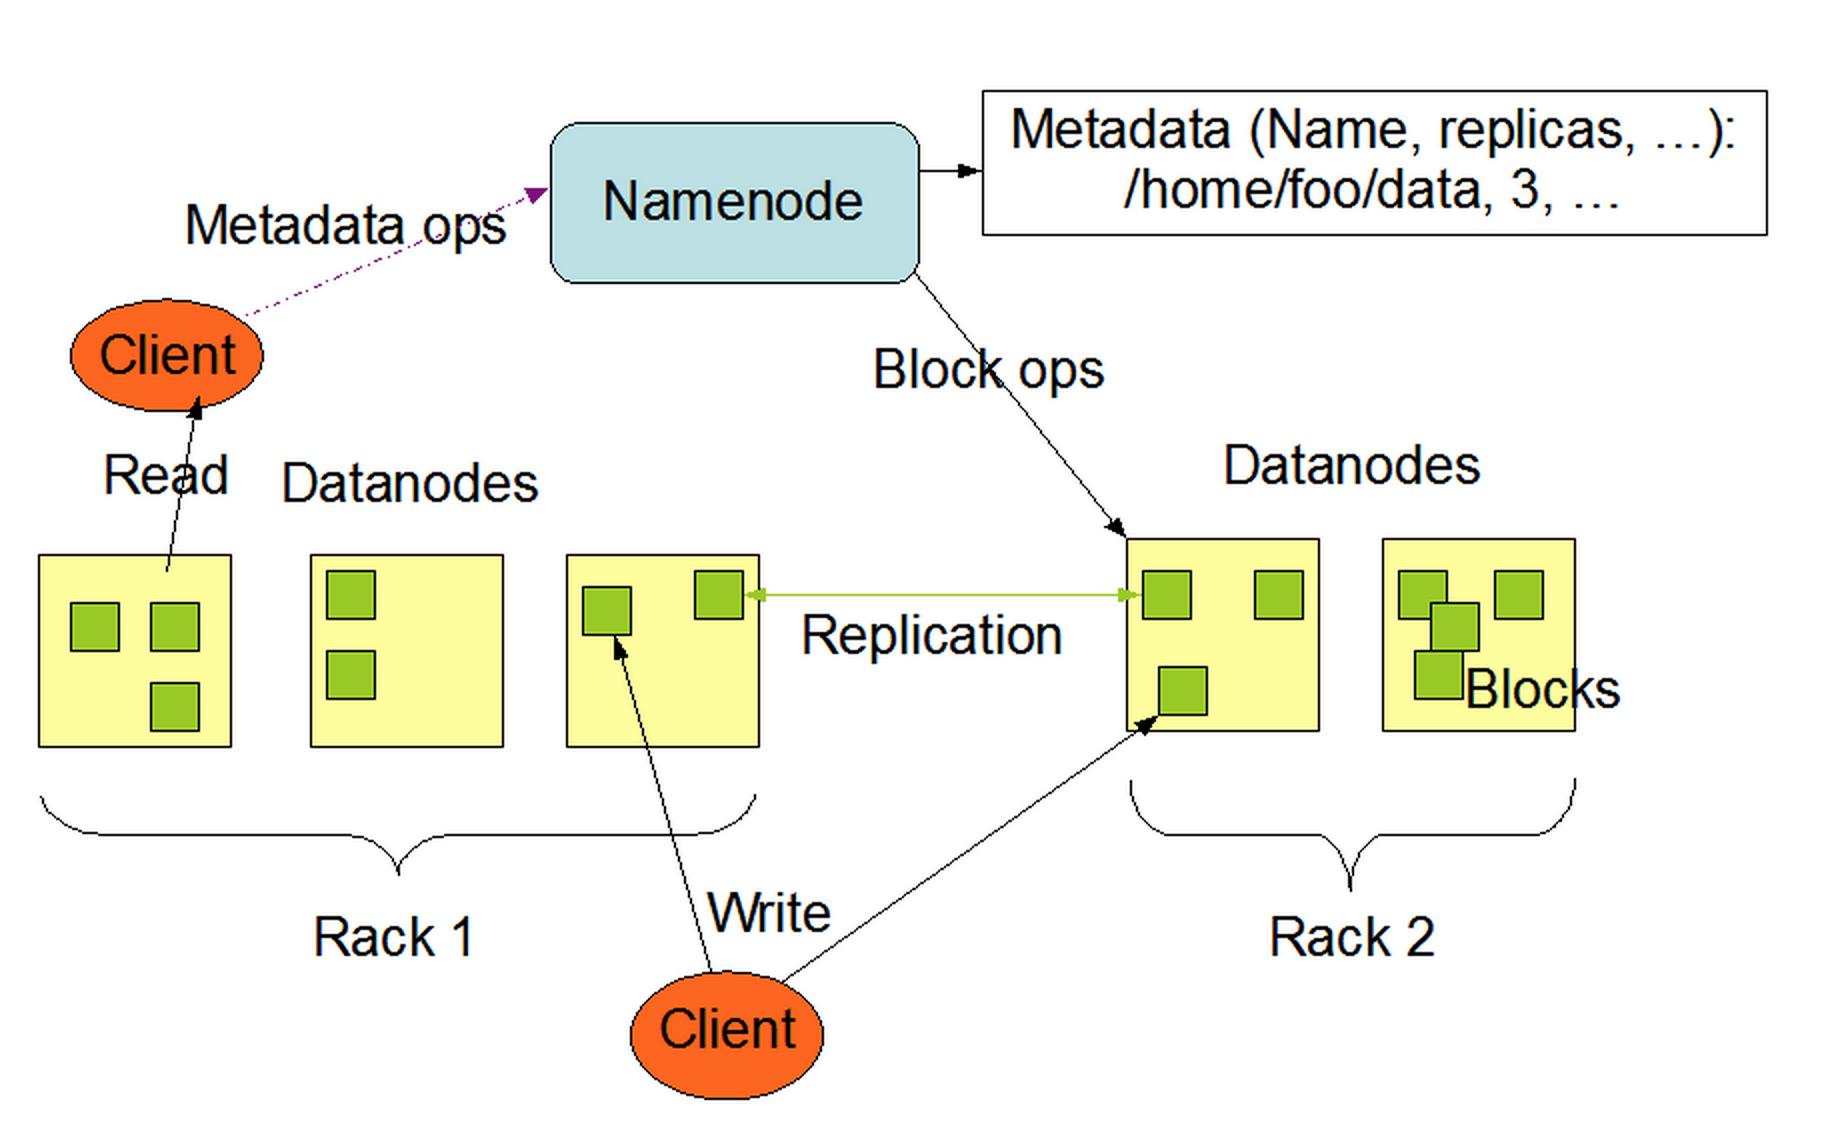
\includegraphics[width=12cm]{imgs/hdfs-architecture}
\caption[HDFS architecture]{HDFS architecture\protect\footnotemark}
        \label{hdfs-1}
\end{figure}
\footnotetext{http://hadoop.apache.org/docs/r2.7.0/hadoop-project-dist/hadoop-hdfs/HdfsDesign.html}
A Namenode holds the namespace of the filesystem, i.e. information about the structure of the filesystem and metadata about the distribution of the files over the datanodes, and listens for client requests such as writes or reads. Datanodes are the worker nodes: they store data and they serve the actual client requests, providing for data in case of read requests or allocating space in case of write requests. In this architecture, Namenode represents a single point of failure, the namespace is kept in memory by the Namenode and it case of its failure all data is compromise. There are several solutions to run HDFS in \textit{High Availablility (HA)} mode such a maintaining a \textit{StandBy} replica synchronized with the master through a network file system \cite{bib23}\\
A file in HDFS is split in several blocks according to its size (HDFS handles block of 128Mb by default), distributed and replicated across the Datanodes according to a per-file policy. The position of each blocks and their replicas are kept in Namenode's namespace. Having a block abstraction gives robustness and fail-tolerance to the storage system in case of Datanodes failure: client requests are normally redirected to the nearest healthy Datanode containing the required information.
\subsection{Oozie}
Apache oozie\cite{bib20} is a workflow scheduler for Hadoop. Each workflow is composed by a sequence of action executed in sequential mode, which means that an action can't be executed until the previous one ended. If configured with YARN resource negotiator, Oozie runs each job in a container context [\ref{yarn}].
Oozie workflow builds a DAG (direct acyclic graph) structure and is composed by a sequence of two possible type of \textit{nodes}:
\begin{itemize}
\item control flow: nodes that control the start, the end and the execution of the workflow without executing any concrete action. Example of this nodes are: start control node, end control node, kill control node, fork control node.
\item action: nodes that execute a task. The actions supported by the latest version (4.2.0 July 2015) are Map-Reduce, Pig, Java, Fs (filesystem), ssh, Spark	 
\end{itemize}
Jobs are scheduled by the server with a minimal granularity of minutes. It is possible to specify an input and an output directory where to read data needed to the job and where to store an eventual result. Moreover, the input and the output directories paths can be expressed in a dynamic way using time  expressions which are evaluated differently according to when the job is executed. All the configurations are submitted to the server using XML files containing information about the location of the application executables, directories paths, application arguments and frequency of the jobs. These configuration files are uploaded on HDFS for being accessible by any node in the cluster.

\section{Spark}
Apache Spark is a distributed framework for batch data processing. It is based on the same paradigm of Hadoop/Map-Reduce, where the computation is split across several nodes in the cluster (\textit{map}) and the final result is given by aggregating the intermediate ones (\textit{reduce}). Spark has been designed for the class of applications which need to iterate several times on the same dataset, such as machine learning and interactive analytics, allowing them to store intermediate data in memory instead of recompute it at every step. For these type of applications, it has been showed how spark outperforms a classic map-reduce paradigm by 10 times \cite{bib21}.\\
In order to be executed in a distributed mode, Spark needs a cluster manager for resources allocation across all the nodes. Spark provides its own standalone cluster manager even though YARN or Mesos can be used. The architecture is composed by a primary node called \textit{driver program} and a set of worker nodes running \textit{executor} threads. When an application is submitted to the cluster, the driver program spreads it across the worker nodes and schedules task to be run by each executor in an independent context (each executor runs its own JVM). In this way there is complete isolation between several applications running on the same cluster, the drawback is that executors belonging to different applications can't share data between themselves and also within the same application they need the support of the driver program for sharing data using special objects such as \textit{broadcast} and \textit{accumulator} variables.

\begin{figure}[h]
        \centering
        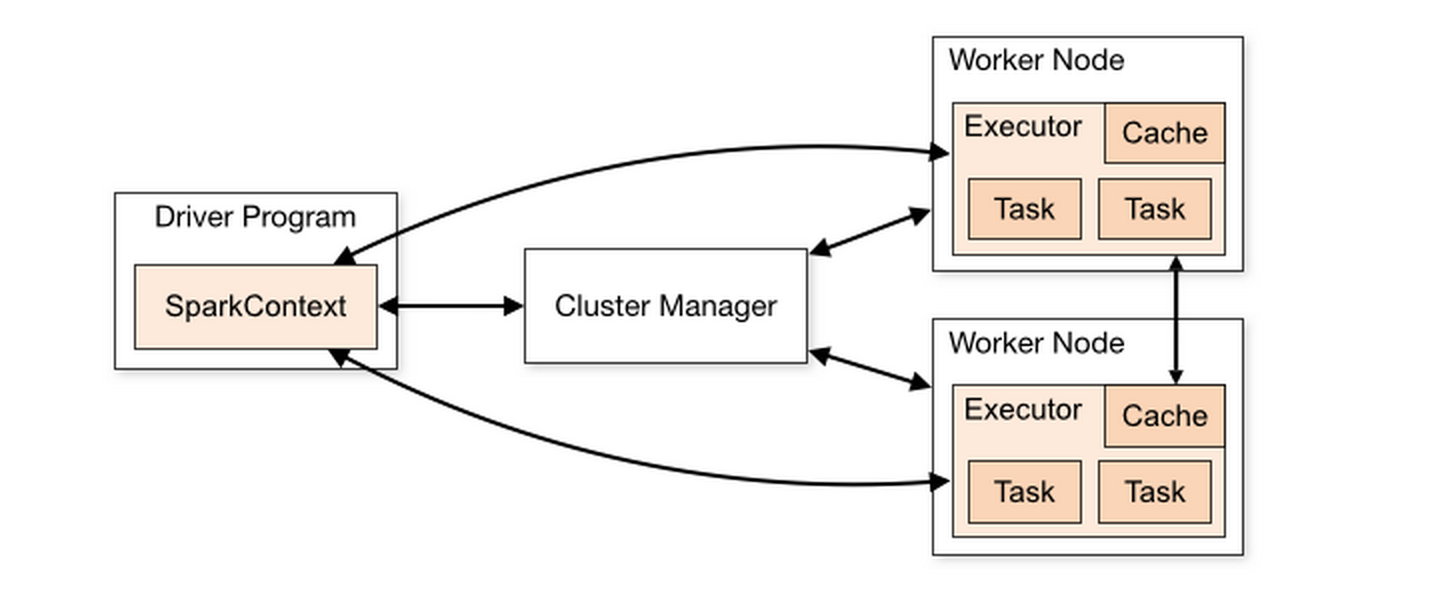
\includegraphics[width=12cm]{imgs/spark-architecture}
\caption[Spark cluster architecture]{Spark cluster architecture\protect\footnotemark}
        \label{spark-1}
\end{figure}
\footnotetext{https://spark.apache.org/docs/latest/cluster-overview.htmld}
The main concept around Spark is an abstraction over a physical dataset called \textit{RDD} \cite{bib8} (resilient distributed dataset). RDDs are read-only, fault-tolerant parallel data structures divided into one or more partitions across a set of machines. They can be created from physical files, parallelizing a collection of elements or modifying an existing RDD by applying a transformation (map, filter...) or an action (reduce, count...). RDD are lazy by nature, in the sense that the driver program keeps in memory the list of transformations needed to compute it rather than execute them at each step. Only when an action requires the RDD to be returned to the driver program, the list of transformations is applied. By default, each transformed RDD is re-calculated each time an action runs on it. It is possible however, to cache it in memory for faster successive accesses. This abstraction increases the robustness of the data model: in case of a partition failure, it can be reconstructed by applying the list of transformations and actions from the last RDD available in memory.

\section{Storm}
Apache Storm is a distributed real-time data processing framework created by Nathan Marz (the proposer of Lambda architecture). Storm considers the data as a stream of \textit{Tuple}, generated in special component called \textit{spouts} and processed by one or more \textit{bolts}.\\ Spouts and bolt can be combined in a direct graph structure called \textit{topology}. Each component (spout or bolt) can be replicated for load distribution. \\
A Storm cluster is composed by a master node and one or more worker nodes. The master node runs a process called \textit{Nimbus}: it handles applications submissions and it is responsible for distributing the code across the nodes, assigning tasks and checking for failures. The worker nodes run one or more processes called \textit{supervisors} in charge of communicating with the master and of executing worker processes.
\begin{figure}[h]
        \centering
        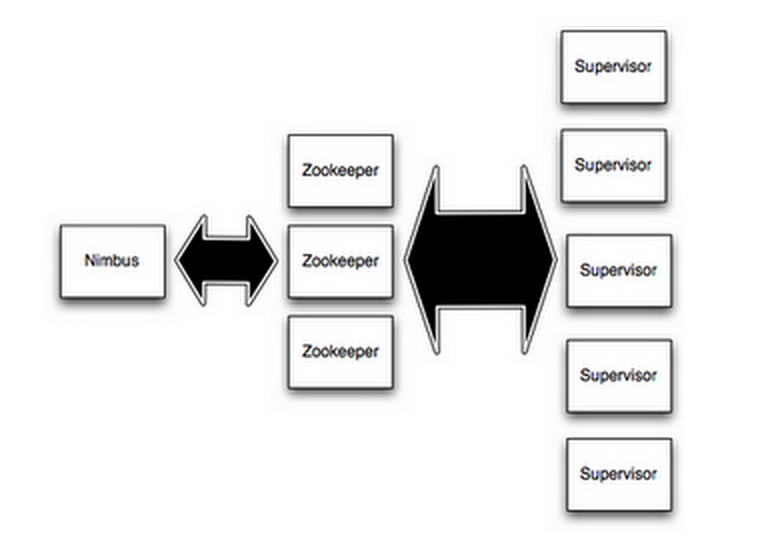
\includegraphics[width=10cm]{imgs/storm-architecture}
\caption[Storm cluster architecture]{Storm cluster architecture\protect\footnotemark}
        \label{storm-1}
\end{figure}
\footnotetext{https://storm.apache.org/documentation/Tutorial.html}
Within a worker process it is possible to run one or more \textit{executor} threads , each \textit{executor} finally runs one or more tasks, with are just parts of the topology belonging to the same component.
As stated before, the main abstraction in Storm the stream of Tuple. Data flows from a component to the next one according to a partition policy: data can be distributed in shuffle mode, by a key, towards a unique component or replicated. Each mode fulfils a different use case: for instance a key-partition (\textit{fields grouping}) is useful when we want to count the occurrences of a particular element in the data stream while a shuffle partition(\textit{shuffle grouping}) is a better approach when the same operation can be performed on each tuple, independently of the actual content of the tuple itself.\\
Storm guarantees by default a \textit{at-least-once} message processing semantic. A topology can be launched with acker components, responsible of ensuring that a tuple is successfully processed within a timeout. Storm keeps in memory a DAG for each tuple generated by a spout: each node in the DAG represents a component which is supposed to process the tuple and sends an ack on success. If the acker receives all the acks for a tuple then that tuple is said to be fully processed, otherwise the tuple is considered failed and the spout responsible for it should be able to regenerate it. In this way no data loss is guaranteed, but a tuple might be processed more than once. 

\section{Elasticsearch}

Elasticsearch is a distributed full-text search engine built on top of Apache Lucene. It provides a set of Rest API for documents indexing, querying and real-time analytics. In order to give a better understanding of how documents are organized inside a cluster, it is possible to compare Elasticsearch structure to a relational database where:
\begin{itemize}
\item a database is called \textit{index}
\item a table is called \textit{type}
\item a table row is a \textit{document} in JSON format
\item a table column is a \textit{field}
\end{itemize}
Elasticsearch uses Lucene's inverted index data structure for fast full-text searches. Basically an inverted index stores, for every unique word inside each document, a list of records that contain that particular word. Furthermore, each word can be normalized according to a text analyzer: for instance it can be converted to a lower case, or in a singular form, if it is a verb it can converted to the infinitive tense, or words can be aggregated if they are synonyms. This step is crucial for having a fast search engine and the user can tune it according to its use cases.\\
Elasticsearch provides a simple master/slaves cluster architecture: either a master or a slave node is capable of indexing or querying documents, the only difference is that a master node is responsible for coordinating operations such a creating an index or adding/deleting a node in the cluster.\\
It is worthy mentioning that an index is just an abstraction for one or more physical data space called \textit{shards}. At index creation time, the user can specify in how many shards to divide it, and how many replicas for a single shards. This is an important setting since the number of shards can't be changed as long as the index is active, only the number of replicas is dynamic. Every time a node leaves or joins the cluster, the master node balances the shardes and the respective replicas over the actual cluster composition.

\chapter{Architectural design}
\label{chap:chapter3}

\section{Case: Vimond Media Solution}
Vimond Media Solution \cite{bib1}, the company at whitch this thesis project was carried out,  is an OTT (Over-the-top) services provider company headquartered in Bergen, Norway. Having customers spread around the world, Vimond is one of the leader in the streaming media market. They provide for a suite of software application called Vimond Media Platform which helps content owners, broadcasters and distributors to manage their online video services. It provides top features such as Rest API, multi-tenancy support, multi-language metadata and much more.

\subsection{Vimond current architecture}

Vimond architecture (figure \ref{vimond-1}) is based of a set of microservices communicating with each other via a publish-subscribe module implemented with Apache Kafka. Using a microservices-based architecture improves modularity and scalability of the whole platform. Content providers interact with the platform with a component called Vimond Control Center, which allows them to ingest, manage and distribute their assets. End users instead, access those assets via an API abstraction over the microservices, after being authenticated with O-Auth protocol. At the moment, relevant actions such as subscription purchase or asset playing performed by end-users are just stored into Cassandra and Oracle databases and used only when needed, for instance when customers request usage reports. What it missing is an independent module for gathering and analyzing these data, possibly in real-time with support for historical data. Lambda architecture seems perfect for defining such a module and in the rest of this chapter we are going to show and describe the proposed framework for this problem.

\begin{sidewaysfigure}
\centering

        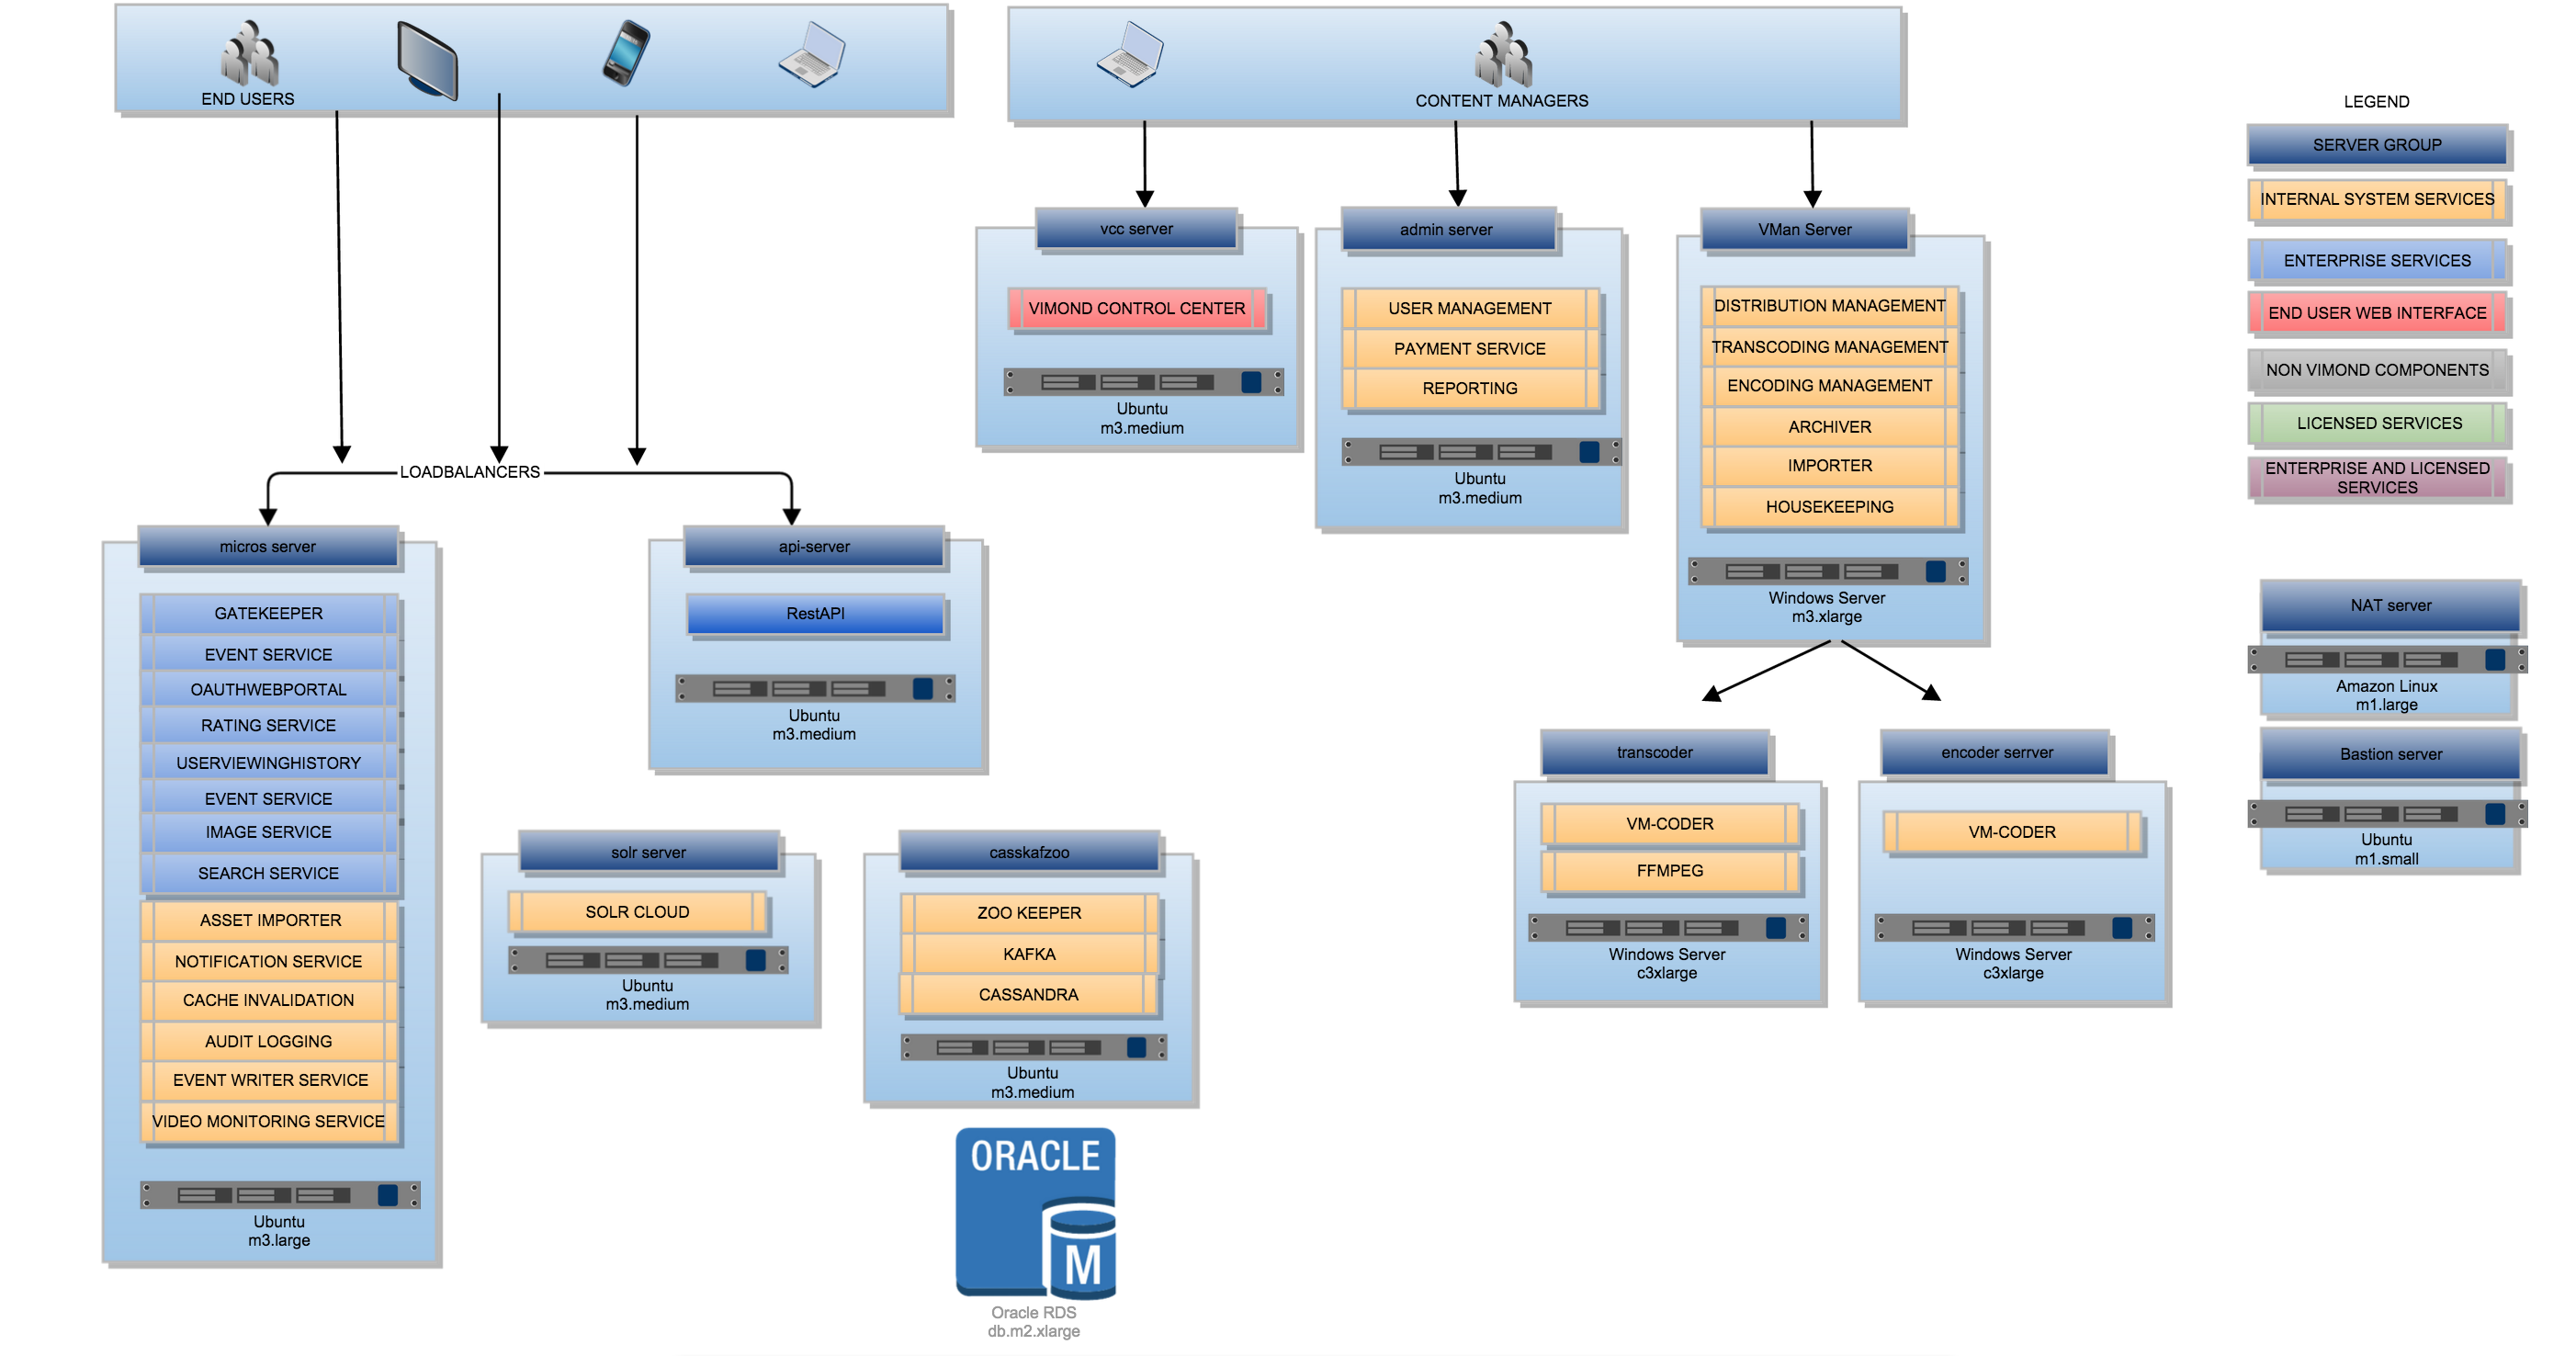
\includegraphics[width=20cm]{imgs/vimond-architecture}
\caption[Vimond architecture example]{Example of Vimond production envirovment.}
        \label{vimond-1}
\end{sidewaysfigure}

\section{Proposed solution}
The proposed solution is meant to be a prof of concept of Lambda architecture, rather then an effective production-ready system. It aims to improve the theoretical idea by simplifying it where there are the majority of problems (i.e. the complexity), resulting still in a three layer architectural pattern. For the rest of the report we will refer to this model as VimondAnalytics.\\
The main simplification comes when dealing with intermediate views. According to the original Lambda architecture pattern, each processing layer produces intermediate views to be merged into global ones in the serving layer. The model we are going to propose avoid storing intermediate views in different databases, data instead are ingested directly in the serving layer. The purpose of the latter is similar to the original one as it has to merge data coming from the two different processing layers, but now, instead of merging views, it merges raw data coming from the real-layer and aggregated ones from the batch layer. The simplification is hence obvious: there is no need anymore for different storage solutions which have different requirements and therefore different problems. All the complexity is moved to the serving layer while the real-time and the batch layer fulfill only to processing requirements. \\

\begin{figure}[h]
        \makebox[\textwidth][c]
        {
        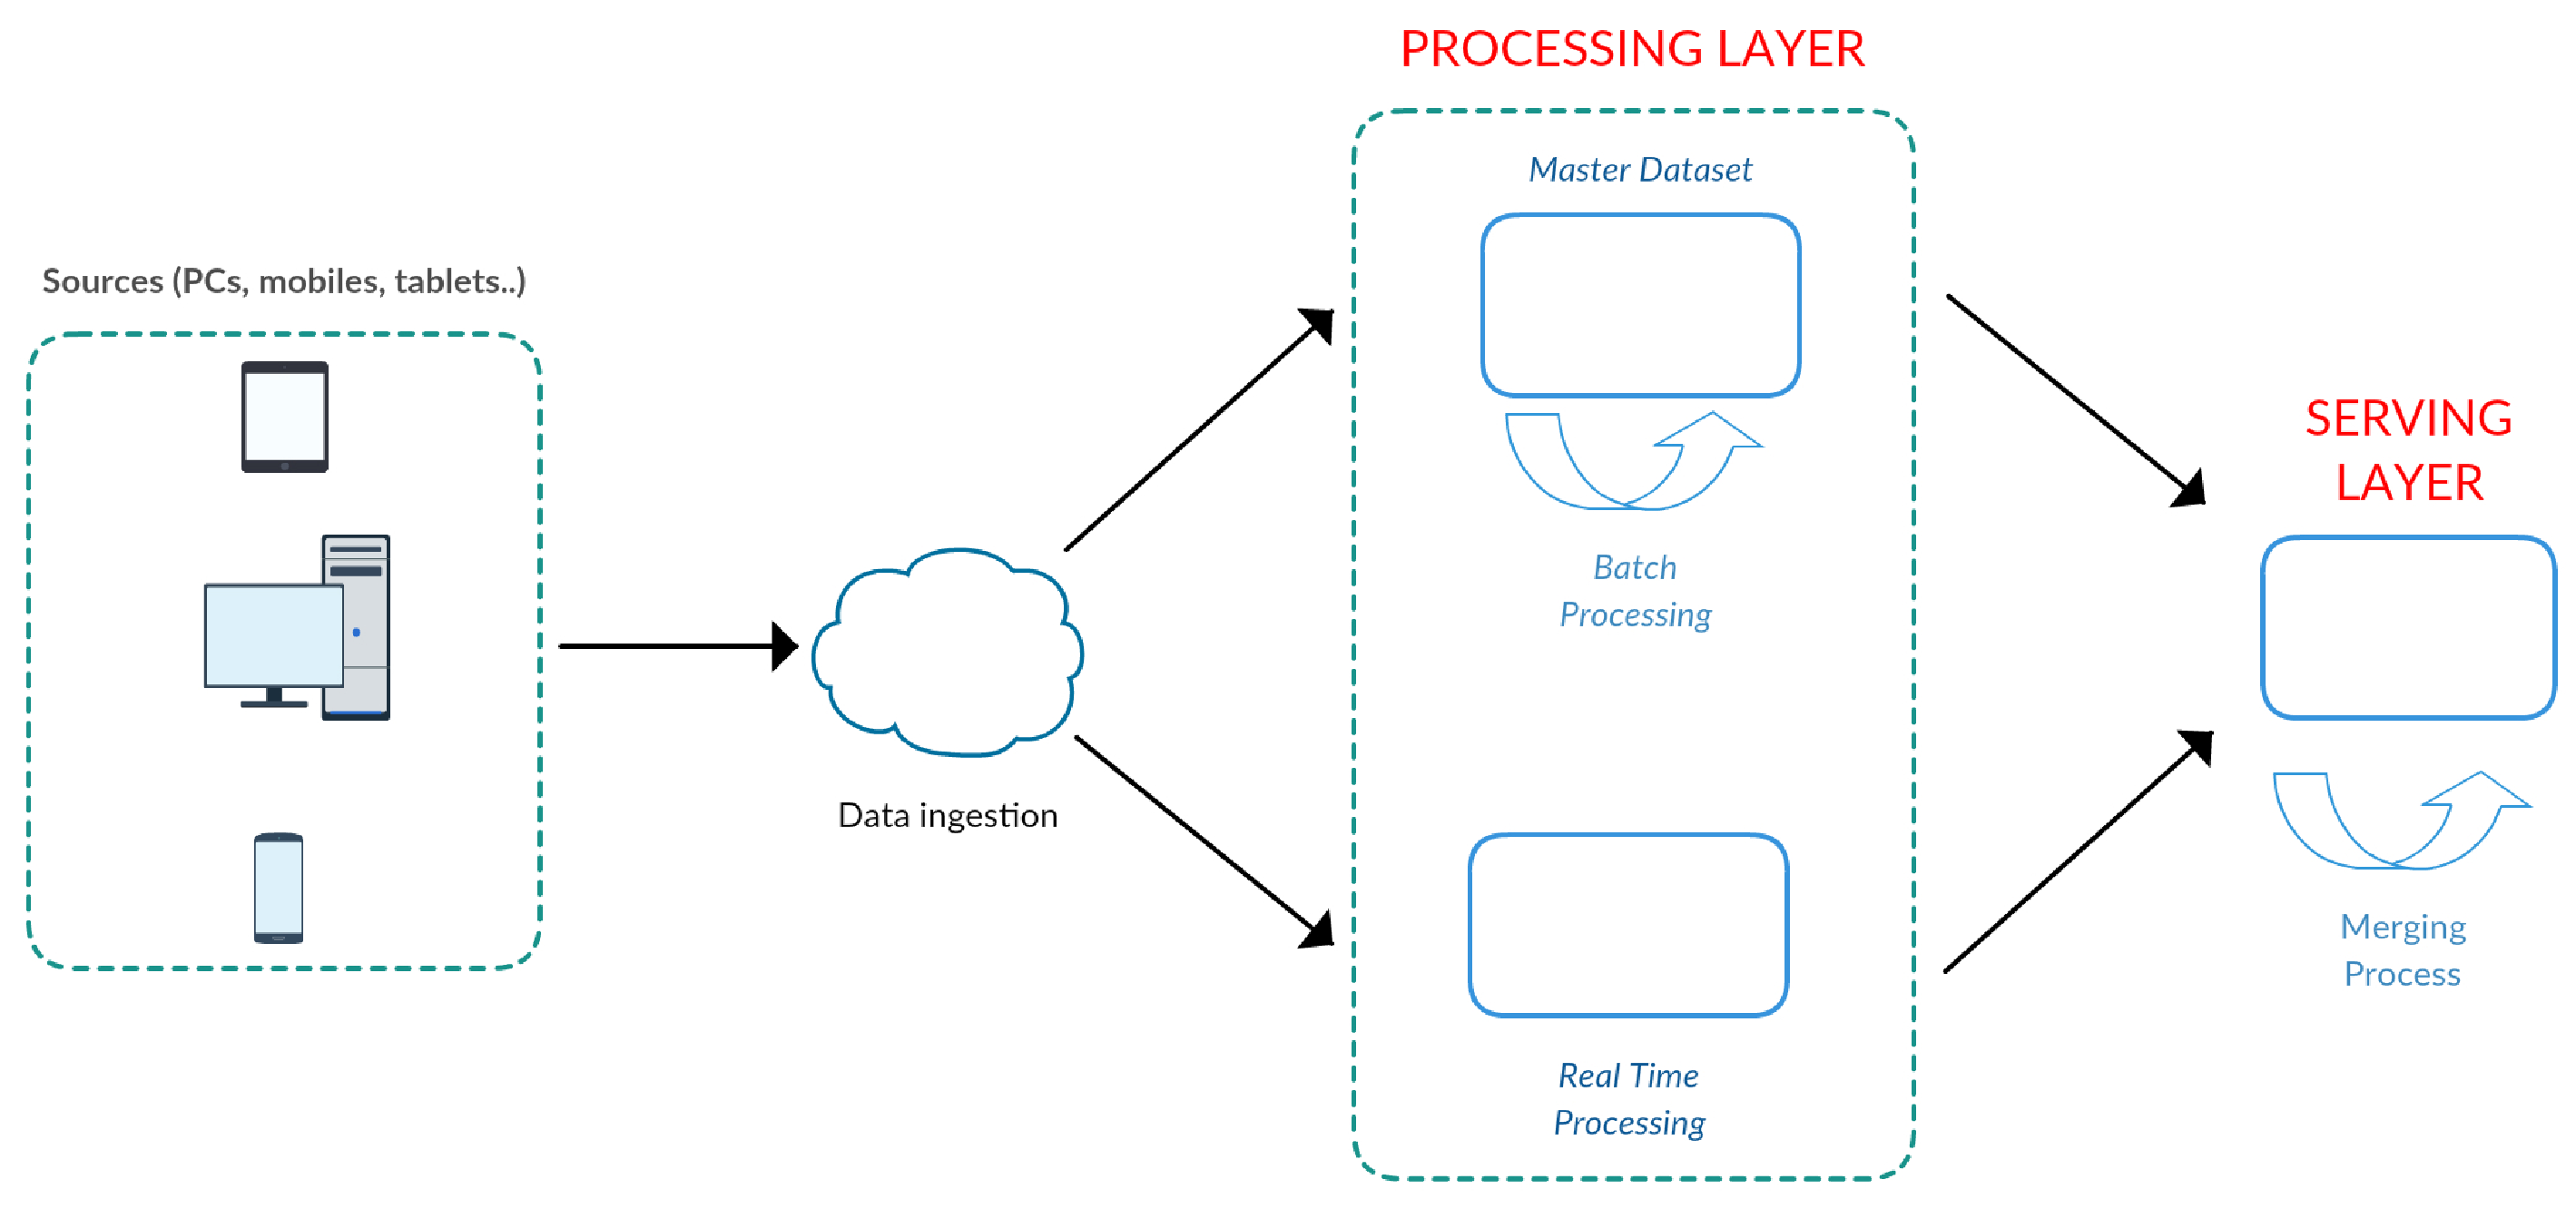
\includegraphics[width=17cm]{imgs/vimondAnalytics}
        }
\caption[VimondAnalytics architecture]{VimondAnalytics architecture}
        \label{vimondAnalytics-1}
\end{figure}

The final architecture is again a composition of several layers. Data come into the system through a \textit{data ingestion} layer, implemented with a publish/subscribe architecture. The \textit{real-time layer} gets data from the data ingestion and after few processing steps, stores them in the serving layer. The \textit{batch layer} stores data in a data lake structure and runs aggregation processes for obtaining compact (and shorter) views out of them, which will be eventually stored as well in the serving layer. The latter aggregates raw data and merges them with the batch ones in order to answer to end-users queries.\\
The rest of the chapter describes each separate layer of the model above briefly introduced.

\subsection{Data ingestion}
Data ingestion layer represents the entry point of the system, where input data are managed and replicated into the batch and the real-time layer. Apache Kafka fits perfectly into this role, as is it handles different consumers and has them fetching messages from different points on the same dataset, according to their capability. \\
In order to get the whole system working we need a data source. Normally artificial dataset can be used for a prof of concept validation but we preferred to use a real one. Vimond provides TV2 Norway with services for its online streaming platform called \textit{TV2 Sumo}. Data used in this project come from that platform and refer to a  player playback functionality which allows a user to resume the stream of an asset when it closes the browser window and wants to re-play from the last point.\\

\subsection{Real time layer}
The real-time layer of this model is very simple, its purpose is to forward data from the data ingestion part to the serving layer after processing them. Differently from the original approach, it does not have to generate any aggregation or storing data on an intermediate database. A possible process executed in this layer could be data augmentation, like IP translation into location and coordinates or user agent breaking into browser and operative system version. Neither an incremental nor a recomputation algoritm is used: augmented data are just written on the serving layer. A typical example of data forwarded by the real time layer could be: 
\begin{listing}
\begin{minted}[frame=single,
               framesep=3mm,
               linenos=true,
               xleftmargin=21pt,
               tabsize=4]{js}
{     
    "eventType": "click"
    "userId" : "12345",
    "targetURL" : "http://www.mywebsite.com/mypage.html"
    "timestamp": "2015-09-06-19:54:00"
}
\end{minted}
\caption{RealTime data example} 
\label{realtimedata-example}
\end{listing}

Apache Storm has been used for implementing this layer as it provides the features we need. No message guarantee policy is required, we are not interested in having a strong consistency level, data need to be moved as fast as possible and a certain degree of inaccuracy is tolerated. Anyway, real-time processing frameworks such as Storm allow to implement an \textit{at-least-once} message processing instead of \textit{at-most-once} where messages loss is possible. According to the use cases of the current scenario, it is possible to switch to the semantic needed.

\subsection{Batch layer}
\label{batch-layer1}
The batch layer is organized in two parts. First data are fetched from the data ingestion layer and saved into a data lake, then they are analyzed and aggregated according to the output views.\\
In order to improve the performances of the fetching process, data are stored in the data lake in batches and two mode of doing it were implemented: 
\begin{itemize}
\item \textbf{unreliable}: the offset for a message is committed after it has been read from the data ingestion layer. This implies that, if the process crashes or fail to write the message on the data lake, the message is lost. In addition, if messages are processed in batch, in case of crash of the process, all the batch is lost. This approach implements a \textit{at-most-once} message delivery semantic.
\item \textbf{reliable}: the offset is committed after a batch of messages is written successfully on the data lake. In case of crash of the process, the one who takes over is going to read from the last committed offeset which represent the latest checkpoint. In case of crash of the process after writing the  messages but before committing the offeset, data will be written twice. This approach implements a \textit{at-least-once} message delivery semantic.
\end{itemize}
Data lake is implemented through Hadoop HDFS. As explained in the previous chapter, HDFS implements an abstraction over a distributed data storage such that classic filesystem operations are possible. Data written into the data lake are organized in a time-folders structure: the dataset is a hierarchy of folders where at the top there are the ones representing days, the second level is for the hours of a particular day and the third is for the division of the hour in intervals. It is possible to divide an hour or a day in several intervals but partitions bigger than a day were not implemented. When a new datum needs to be written in the dataset, it goes to the corresponding folder according to its timestamp. For instance,  let assume a partition criteria of 15 minutes: this means that every folder representing an hour contains 4 sub-folders representing the minutes intervals (00-14, 15-29, 30-44, 45-59). The figure \ref{datalake-1} explains where data are actually written in this scenario, according to their timestamp.

\begin{figure}[h]
        \centering
        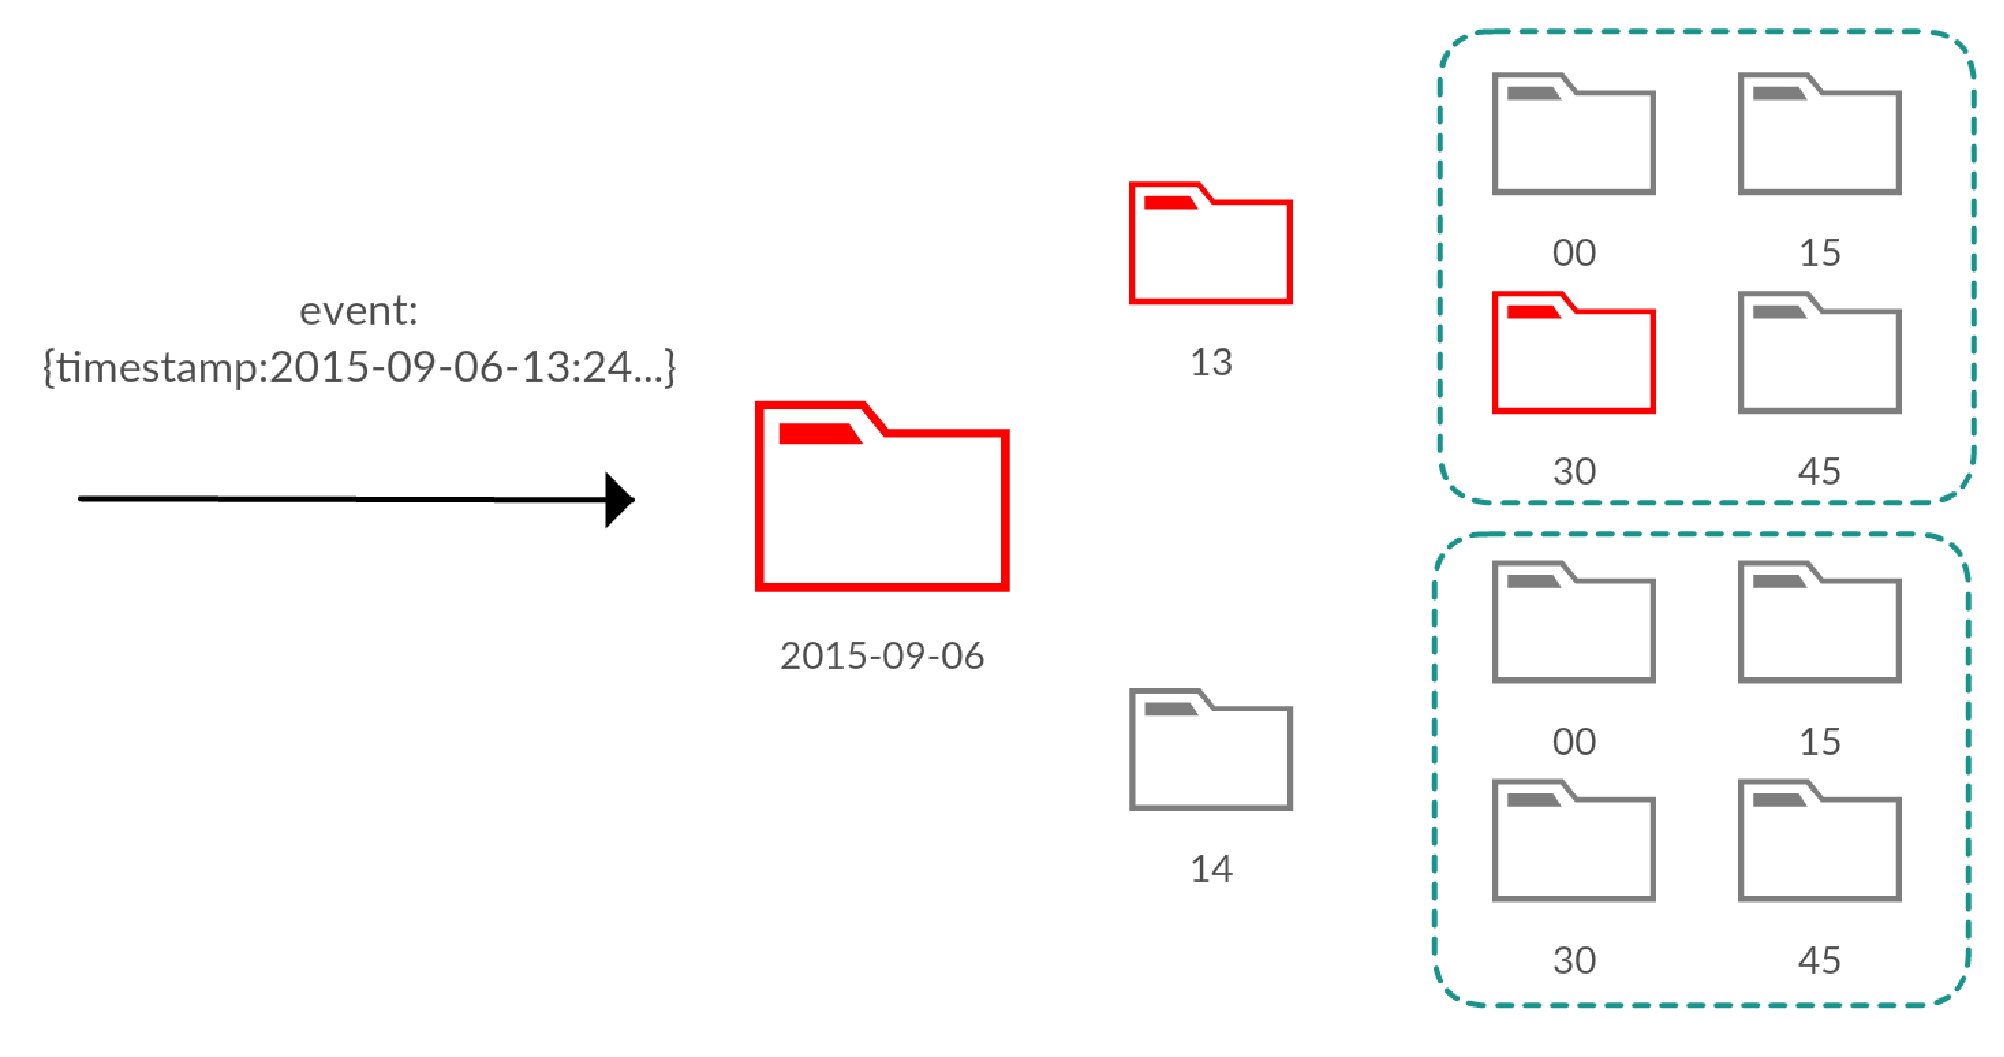
\includegraphics[width=12cm]{imgs/datasetStructure}
\caption[Data lake structure]{Time folder structure: an event is saved in the corresponding folder, according to its timestamp.}
        \label{datalake-1}
\end{figure}

While new data are ingested into the data lake, the batch layer is responsible to execute aggregation processes on the historical ones. Each of these processes takes in input data contained inside a specific folder, which changes over the different executions, and produces as output a set of events representing aggregated data and they are stored directly into the serving layer, without the use of an intermediate database. A typical example of a datum generated by this layer could be:
\begin{listing}
\begin{minted}[frame=single,
               framesep=3mm,
               linenos=true,
               xleftmargin=21pt,
               tabsize=4]{js}
{     
    "eventType": "click"
    "targetURL" : "http://www.mywebsite.com/mypage.html"
    "counter": 100
    "timestamp": "2015-09-06-19:54:00"
}
\end{minted}
\caption{Batch layer data example} 
\label{batchlayer-example}
\end{listing}

An incremental approach can be used, but this model has been thought for a recomputational one over the different data subsets. The different batch views produced at each execution can be aggregated with each others in the serving layer. While this approach simplifies a lot the whole aggregation processes, it has limitations in the type of results it can produce as explained in the last subsection of this chapter.\\
Finally, after a batch window of data has been processed, according to the principles of Lambda architecture, real-time data included in that time window are no longer needed as we have an aggregated version, much smaller and faster to query. It is a duty of this layer ensuring that, after the succesful completion of a batch process, the corresponding real-time data are deleted. In this way, all the approximation made by the real-time layer are eventually corrected by the batch views.

\subsection{Serving layer}
The serving layer of VimondAnalytics presents the biggest differences with the original idea proposed by Lambda architecture. As said in the previous chapter, the serving layer should index the batch views and merge them with the real-time ones. Here instead, we don't have anymore the concept of intermediate views, but only final ones are presented to end-users. For this purpose, it is needed a solution which provides storage and aggregation functionalities.\\
Two kind of data are written into the serving layer:
\begin{itemize}
\item data coming from the real-time layer
\item aggregated data coming from the batch layer. 
\end{itemize}
According to the data example provided in the previous sections, a serving view regarding the count of clicks for a particular web page merges all the real-time data for that webpage with the ones generate from the batch layer, according to the timeframe requested by the query. If the serving layer uses JSON syntax as well, then an output result could be the one proposed in figure \ref{servinglayer-example}.
\begin{listing}
\begin{minted}[frame=single,
               framesep=3mm,
               linenos=true,
               xleftmargin=21pt,
               tabsize=4]{js}
{     
    "eventType": "click"
    "targetURL" : "http://www.mywebsite.com/mypage.html"
    "counter": 200
    "from": "2015-09-06-19:00:00"
    "to": "2015-09-06-20:00:00"
}
\end{minted}
\caption{Serving Layer data example} 
\label{servinglayer-example}
\end{listing}
Elasticsearch was used for implementing this layer. We are not interested in the full-text search engine but we exploited mostly its aggregation functionalities on the documents stored into it. 
\subsection{Considerations}
\label{chap3:consideration}
In this chapter we presented a Lambda architecture based model for big data analytics. The idea behind this model is the simplification of the theoretical one, removing intermediate views and then complexity to the whole system and computing final views in the serving layer, as a combination of raw data and batch results.\\
Concerning the batch layer, looking at the data in time windows causes limitations in the type of results that can be overall computed. Let assume to have two consecutive batch windows of data, created by a time partitioning structure as explained in the section \ref{batch-layer1}. The different results calculated on each window are then stored in the serving layer and aggregated with each others if a query wants to extract data from a time interval containing both of them. Hence, we need to ensure that the aggregated results are consistent among all the different batches, which is, given two partitions \textit{A} and \textit{B} and an aggregation function \textit{f}, the following equation $f(A) + f(B) = f(A+B)$ must hold. For all the other cases where it does not hold, an incremental approach is needed. Example of consistent views are generated by unique events over the time, like a purchase or a content rating. \\
Other limitations of this approach are inherited from the Lambda architecture one: it is not possible to query the system for a time interval shorter than the batch time window. The smaller the granularity, the greater the accuracy of the query, but computing batch jobs more frequently might not be the best option in terms of efficiency, even if applied on a smaller subset of data.\\
The applicability of this framework lies on the use cases where a normal query would investigate what happened in a fixed time span in the past, corresponding to one or more batch windows (for instance, recalling the previous example, the number of clicks for a webpage from 10 am to 12 am, assuming a 30 minutes batch interval), or a real-time overview over all the historical data saved in the serving layer.
\chapter{Implementation}
\label{chap:chapter4}
In this chapter we are going to show a concrete implementation of the architecture explained previously. For each layer we will provide explaination of the most important features using diagrams and code snippets.

\section{AWS Deploy}
elencare le macchine usate e come sono stati deployati i vari servizi su di esse
mettere configurazioni?

\section{Data ingestion}
TV2 runs Sumo production envirovment into a virtual private cloud on Amazon Web Service (AWS), isolated from the outside network and it is not possible to fetch them directly. A typical cloud production envirovment keeps the virtual machines inside private networks and routes the network traffic to the external network through NAT instances. A bastion server is normally placed as protection against undesidered accesses such that only trusted user can access the private cloud. \\

Since Sumo platform uses Apache Kafka as a message sharing system between several services, it has been convenient and easy to create a "data bridge" inside that envirovment for pushing data inside the VimondAnalytics one. \\
For this purpose it has been used an already existing Vimond project called "Firehose", which has been modified for this use case. Firehose simply implements a two endpoints system. Data are read from a Kafka topic, validated and forwarded to another Kafka cluster. For security reason, Firehose is installed on a machine inside TV2 VPC: in this way the Kafka cluster source is directly accessible throught private IPs. In order to connect it to the VimondAnalytics Kafka cluster, an elastic IP is assagned to the latter.

\begin{figure}[h]
        \centering
        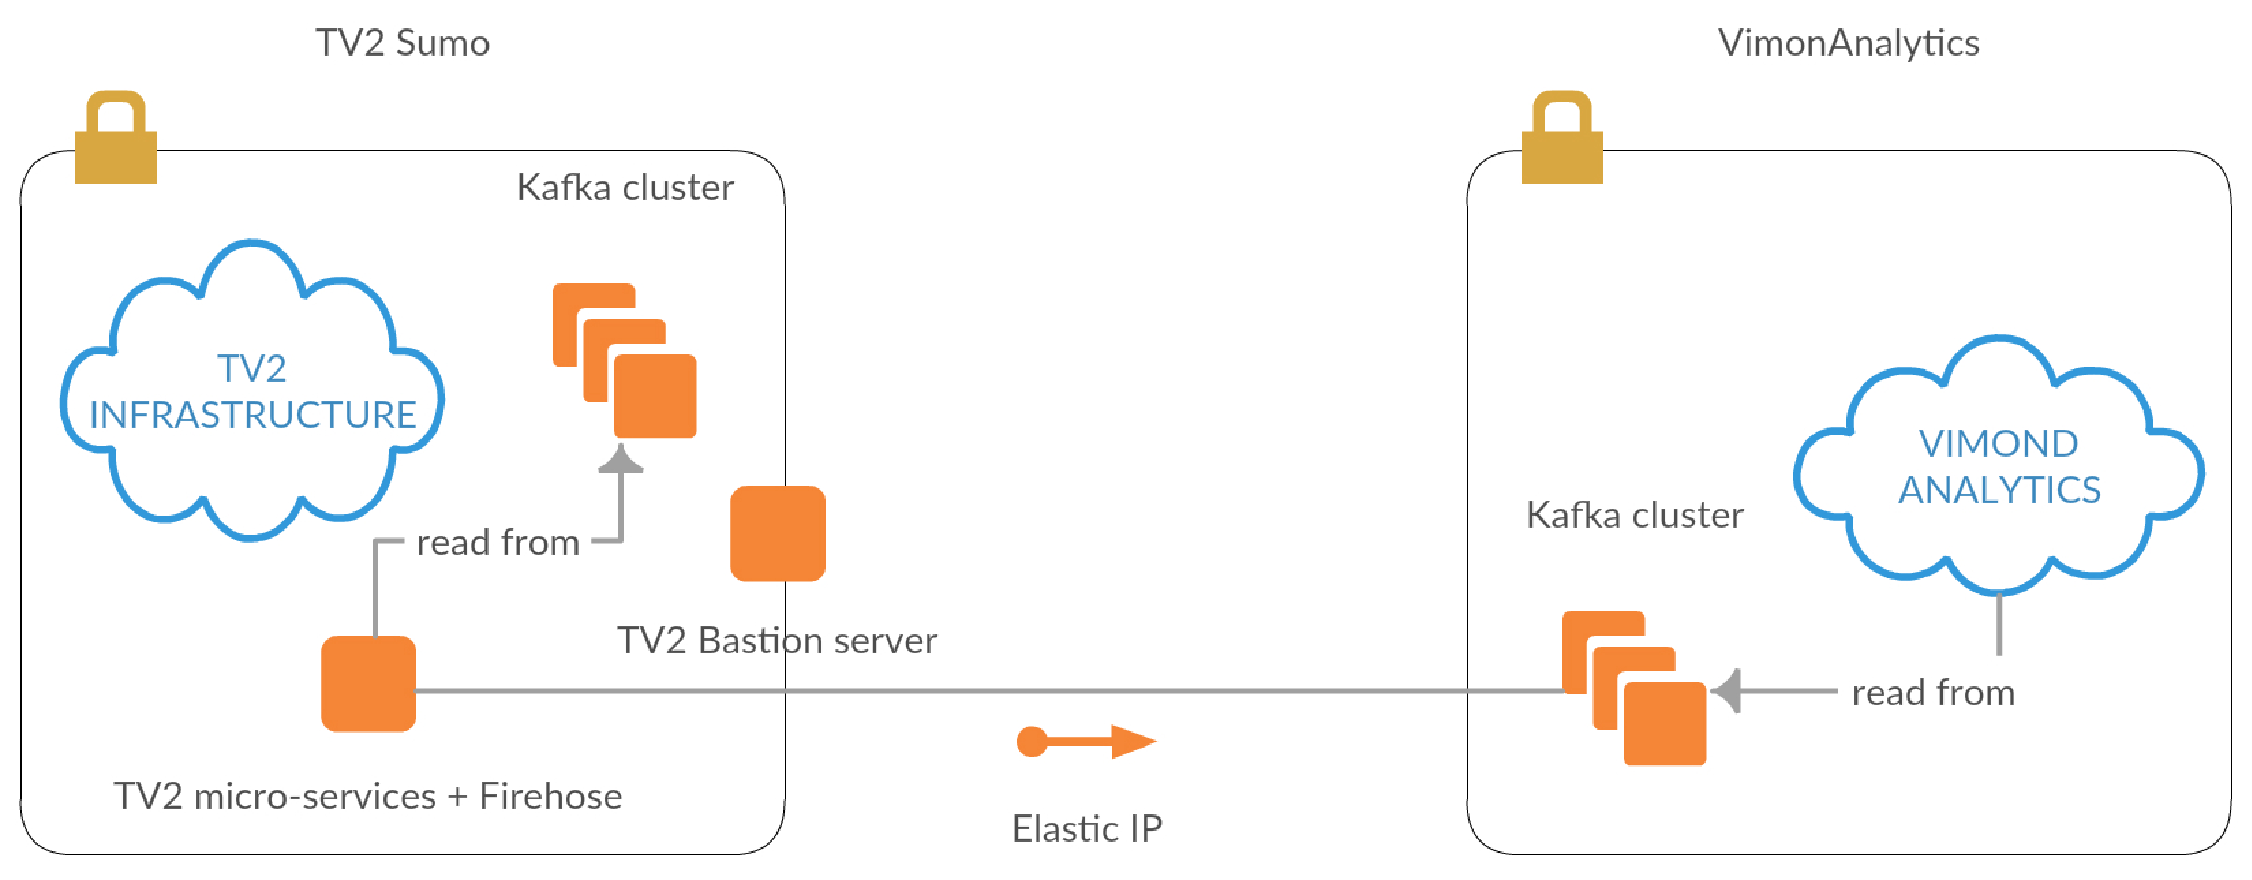
\includegraphics[width=12cm]{imgs/Firehose.pdf}
\caption[Firehose data bridge]{Firehose data bridge}
        \label{firehose-1}
\end{figure}

\subsubsection{Data model}
As said in the previous chapter, the data used for this project come from the resume player functionality provided by TV2 pay-per-view platform \textit{Sumo}. Data are generated by players running on different devices: it results in two type of events according to the usage of silverlight plugin. The events generated by other plugins contains a subset of information of the ones generated by silverlight plugin. Specifically, an example of non-silverlight event is:
\begin{listing}
\begin{minted}[frame=single,
               framesep=3mm,
               linenos=true,
               xleftmargin=21pt,
               tabsize=4]{js}
               
{     
    "eventName":"player_log_event"
    "originator":"player"
    "timestamp":"2015-09-13T10:31:39.879Z"
    "guid":"5d33aa50-8232-447e-8b5a-14b4317f1265"
    "progress":
    {
    	"assetId":958291
    	"title":"God morgen Norge"
    	"offset":
    	{
    		"duration":7133249
    		"pos":7101143
    	}
    	"category":
    	{
    		"id":919990
    		"name":"Innev?rende sesong"
    	}
    }
}               
\end{minted}
\caption{Non silverlight event example} 
\label{nosilveright-example}
\end{listing}

\newpage
In addition to these information, an event generated by silverligth plugin contains an additional field with details about the client used for playing a particular asset. In listing \ref{silveright-example} we reported the most important fields for our analysis.

\begin{listing}
\begin{minted}[frame=single,
               framesep=3mm,
               linenos=true,
               xleftmargin=21pt,
               tabsize=4]{js}
               
{     
    "client":
    {
    	"playerEvent":"period"
    	"userAgent":"Mozilla/5.0 (Windows NT 6.1; WOW64; rv:40.0) 
    	Gecko/20100101 Firefox/40.0"
    	"env.platform":"silverlight"
    	"buildName":"Vimond.Player.TV2Sumo"
    	"video.format":"smil"
    }
}               
\end{minted}
\caption{Silverlight event example} 
\label{silveright-example}
\end{listing}


\section{Output results}
One of the limit of lambda architecture is that the output needs to be defined a priori. Accorting to the considerations made in section \ref{chap3:consideration}, the following output views has been defined:
\begin{enumerate}
\item Number of times of assets starting or ending. 
\item Most started assets.
\item Most ended assets.
\item Most browsers used when starting an asset.
\item Most OSs used when starting an asset.
\item Most video formats used when starting an asset.
\end{enumerate}
In order to have consistent outputs across the different batch views we exploit the field \textit{"playerEvents"} which gives information of the type of event performed by the user. It can assume the values \textit{start}, \textit{period} and \textit{end}. We could not use the event marked with \textit{period} as the different batch windows does not share information and then every results produced out of them would have not been consistent. A \textit{playerEvent=start} or \textit{playerEvent=end} represents instread a unique event. Unfortunately, only a subset of the imput data contains information about the player event (i.e. the one generated by the silverlight plugin). A request has been forwared to TV2 for having these information also in the events generated by other devices. Moreover it has been requested to change the mode of generating \textit{end} events: an user likely stops the streaming of an asset before it actually ends, for instance when skipping the ending titles, and this results in a smaller number of this kind of events. An alternateve solution would be to consider an asset to be ended when the streaming reached a certain percentage over its lenght, for instance 95\%. These features are going to be implemented within the next platform release.

\section{Batch layer}

\subsection{EventFetcher}
EventFetcher is the process in charge of reading events from Kafka a store them in the HDFS according to their timestamp. There are two different execution mode: unreliable and realiable. Figure \ref{EF-Class} shows the class diagram for the main classes involved, reporting the most important fields and methods.
\begin{figure}[h]
        \centering
        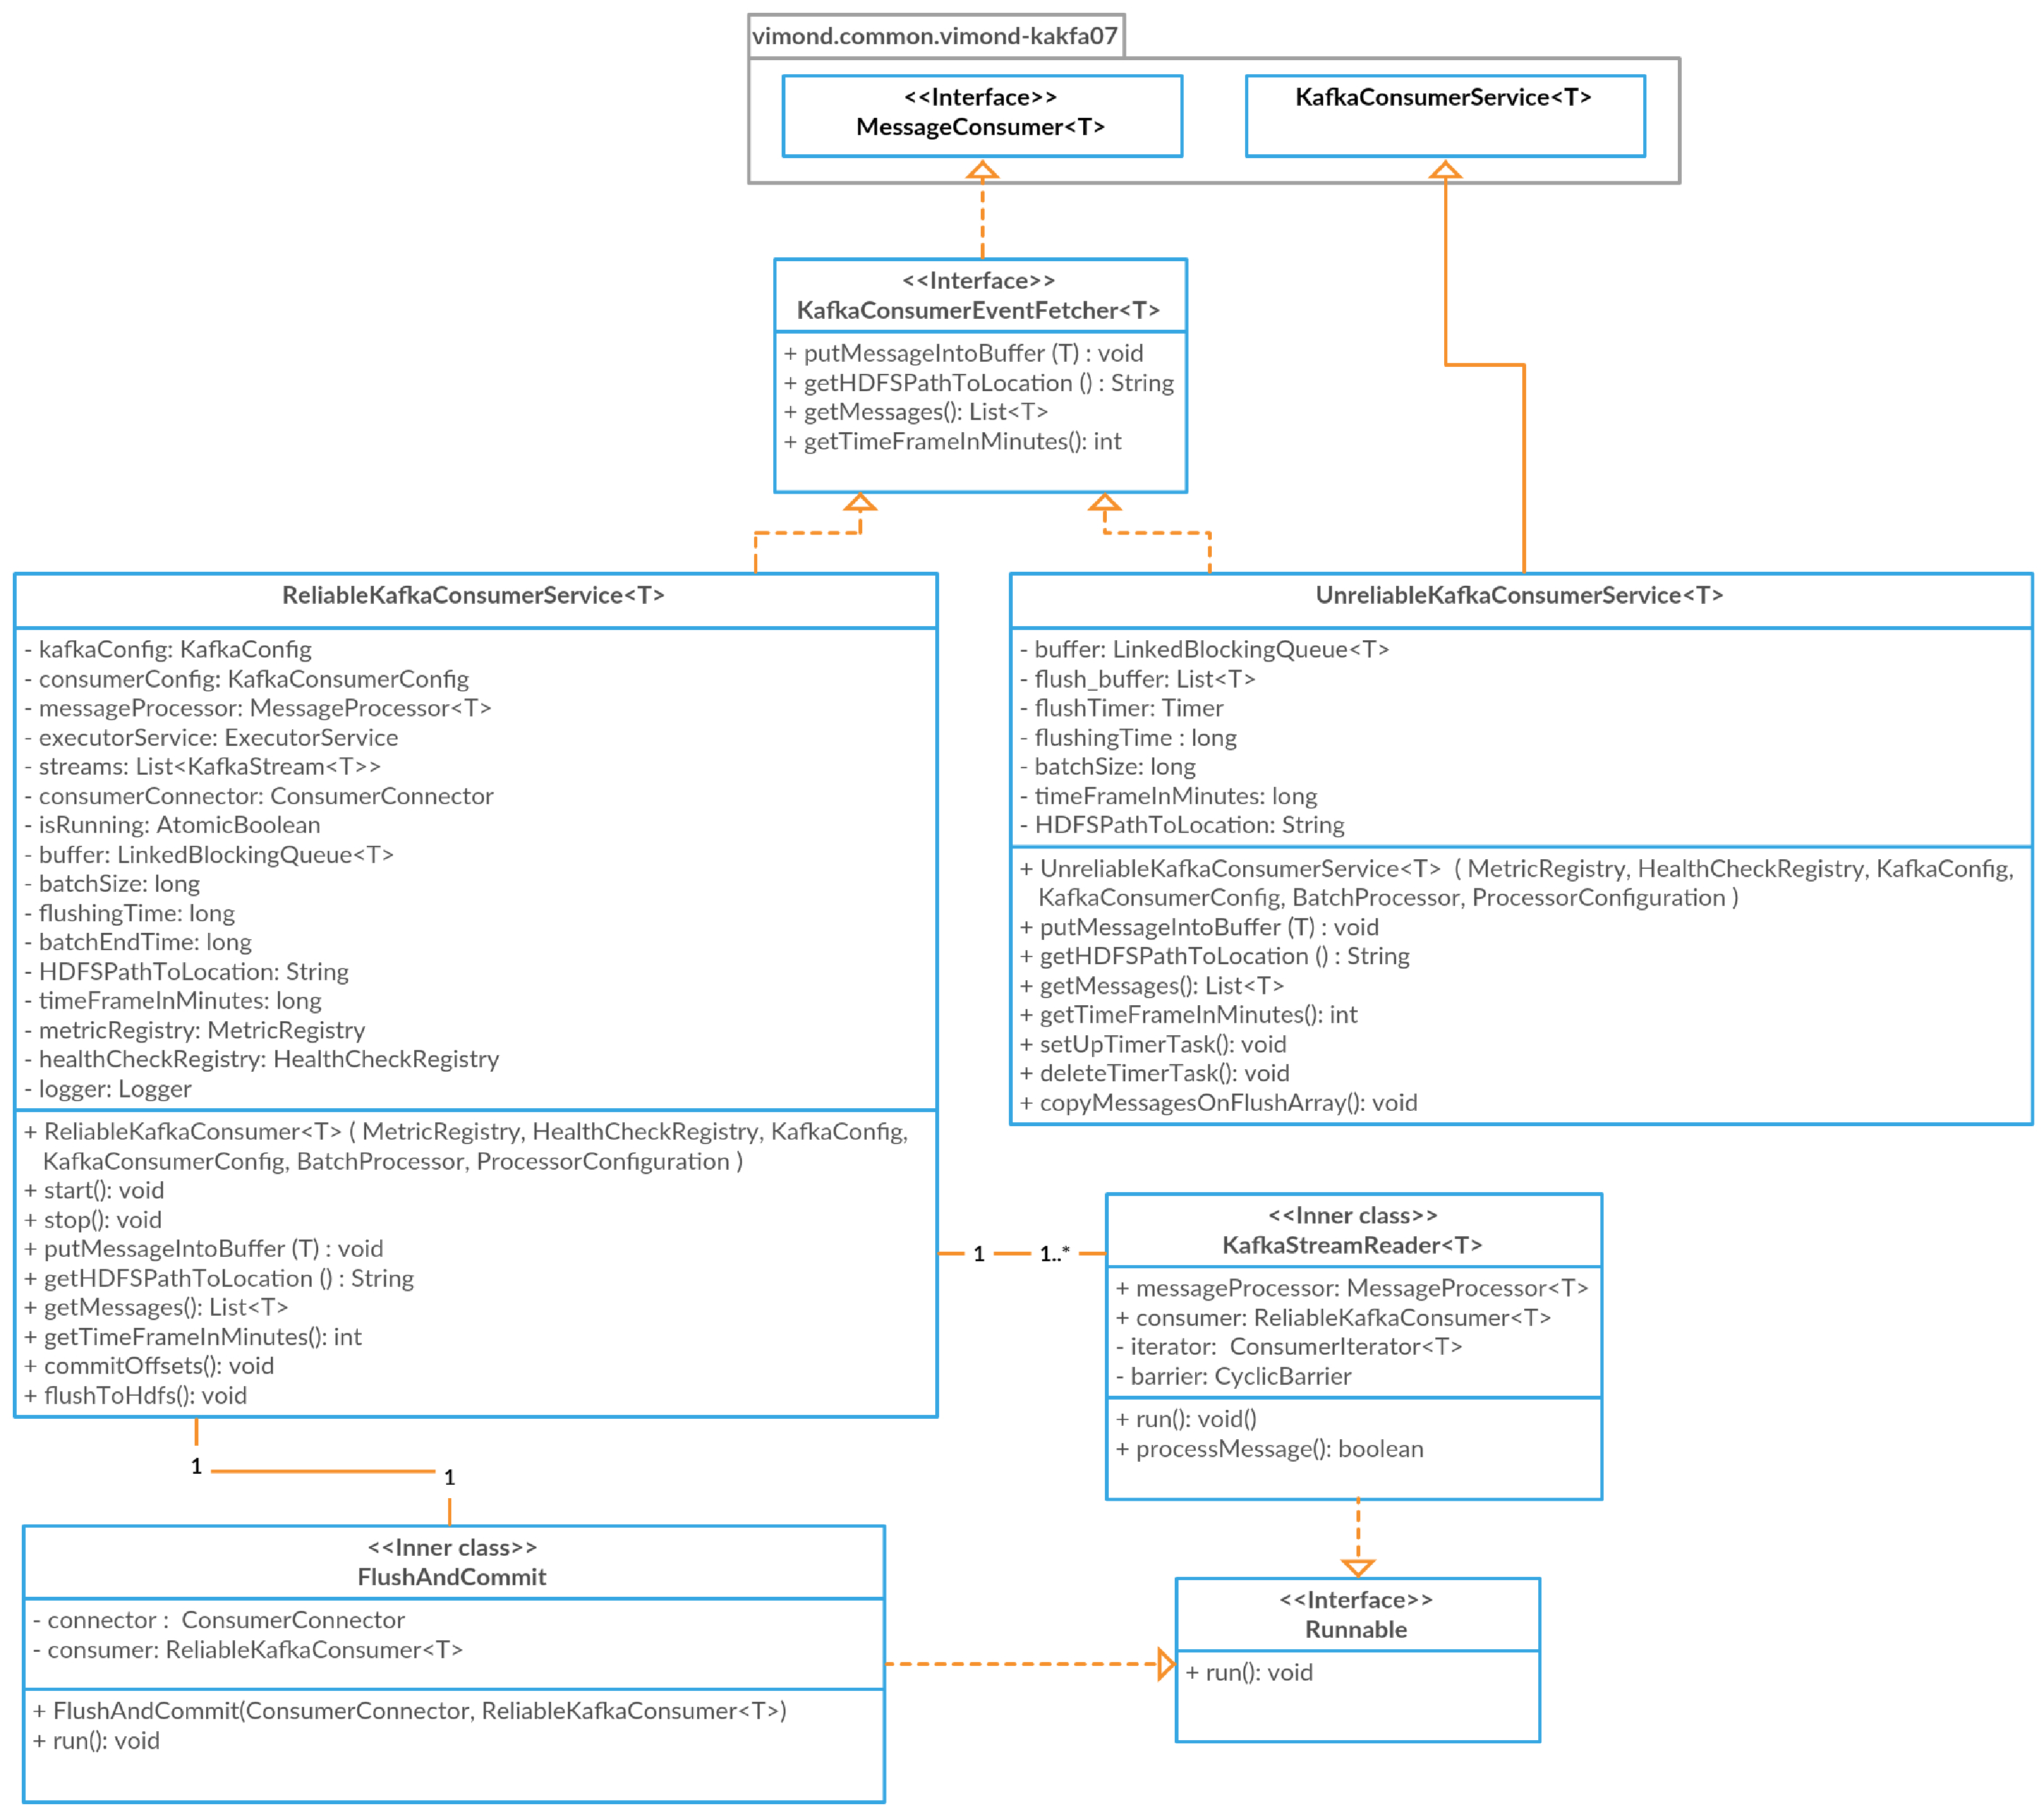
\includegraphics[width=15cm]{imgs/eventfetcher-uml}
\caption[EventFetcher class diagram]{EventFetcher class diagram}
        \label{EF-Class}
\end{figure}

The \textit{UnreliableKafkaConsumerService} extends a kafka consumer class defined in the Vimond repository since the latter offers method for reading messages from a kafka brokers and committing the offset immediately after. What was missing was the ability to process the messages in batches. Each consumer threads reads from kafka and puts the message in a \textit{LinkedBlockingQueue}. The usage of this object is due to its thread-saftness. Each batch operation is triggered either by time or by a threshold on the number of messages stored in memory. Whenever one of this events occurs, the messages are copied into a separate buffer and written in batch into the HDFS from a separate task. This ensure that the storing messagest is not a bottleneck in the overall process, but does not give any guarantees about the correct execution of the operation since the consumer threads are not aware of the writing one.\\
The \textit{ReliableKafkaConsumerService} instread, behaves similarly to the unreliable counterpart, but does not commit a message offset after reading it, only when a batch has been successfully written on HDFS. All the consumer thread are synchronized by a \textit{CyclicBarrier} object. Every time a message is reveived, it is stored in a common buffer and each consumer thread checks if the message threshold or a batch interval has been reached and in case blocks itself on the barrier. The last thread to complete these operations is the one delegated to write the messages into the HDFS: it first tries to contact the HDFS namenode and, in case of its availability, it proceeds with the writing part. In case the namenode is not available, for instance due to a network error, it keeps retrying to contact it using an exponential backoff policy. When the writing process is completed, the offset is finally committed since that batch of messages is considered processed. In order to avoid deadlock, the other threads waits on the barrier for no more than a configurable time, after that, the overall programs raise an exception and exits. This is not the best approch even though guarantees that the next execution of the program reads the same messages that otherwise could have been lost. 

\subsection{Batch data pipeline}
As we said before, we used Apache Spark for implementing this layer. Spark itself does not provide any scheduling mechanism but just a single execution of the aggregation process. Normally an action scheduler is needed for the repetition of the same batch job, each time parametrized in a different way. Considering the usage of Hadoop HDFS as a solution for the data storage, it resulted convenient using Apache Oozie, the official job scheduler over Hadoop. As we explained in chapter \ref{chap:chapter2}, Oozie allows to schedule a DAG of actions, where an action is executed only when the previous one ended.\\
\begin{figure}[h]
        \centering
        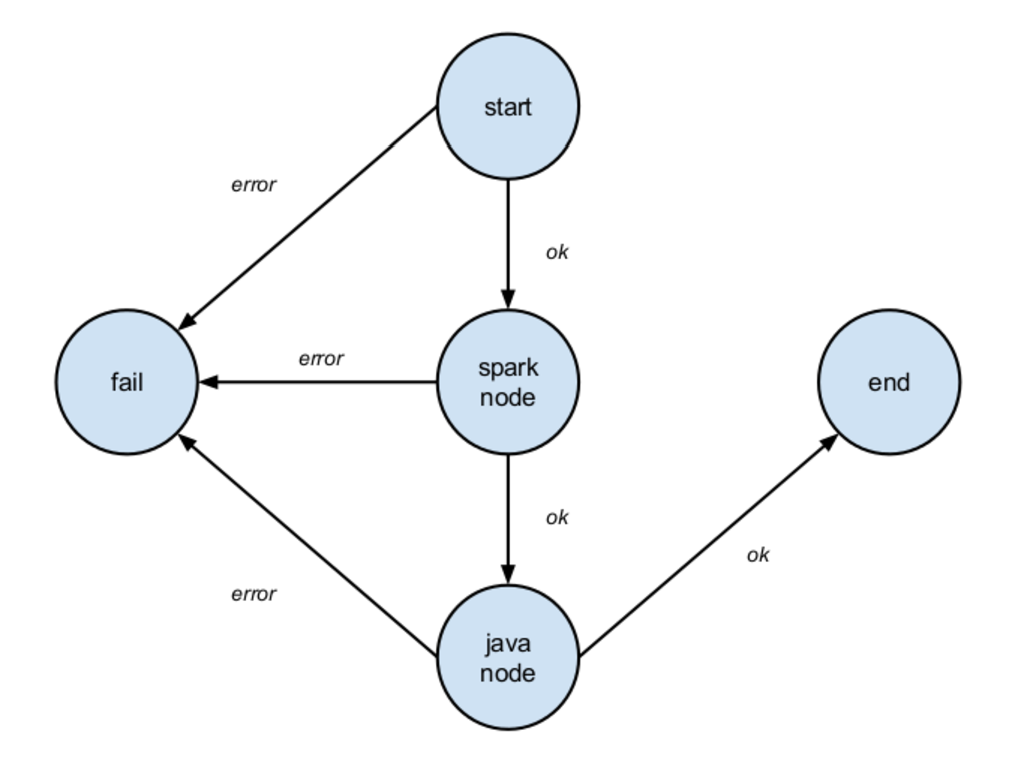
\includegraphics[width=12cm]{imgs/Oozie-DAG.pdf}
\caption[Oozie data pipeline]{Oozie data pipeline}
        \label{oozieDAG}
\end{figure}
Picture \ref{oozieDAG} shows the sequence of actions performed at every execution:
\begin{itemize}
\item start, fail and end are control nodes.
\item spark-node and java-node are action nodes.
\end{itemize}
The user specifies the input parameters such as the beginning time or the frequency of the execution through a property file containing a list of \textit{key=value} tuple.
A execution of the DAG is defined through an XML file called \textit{workflow.xml}, while the scheduling is defined though  a \textit{coordinator.xml} file. Oozie allows to define parametrized paramenter which are resolved with a different value according to the current execution: in this case the job takes a different input folder according to the time of the execution as showed in listing \ref{oozie-example}.
\begin{listing}
\begin{minted}{xml}
<datasets>
	<dataset name="vimondEvents" frequency="${coord:minutes(30)}" 
	initial-instance="${datasetStartTime}" timezone="GMT+02:00">
	<uri-template>${nameNode}/user/${coord:user()}/${datasetFolder}
	/master/${YEAR}-${MONTH}-${DAY}/${HOUR}/${MINUTE}</uri-template>
	</dataset>
</datasets>
<input-events>
 	<data-in name="input" dataset="vimondEvents">
  		<instance>${coord:current(-2)} </instance>
	</data-in>
</input-events>
\end{minted}
\caption{RealTime data example} 
\label{oozie-example}
\end{listing}

With the \textit{dataset} tag it is possible to define a parametric path where to take the data according to the \textit{YEAR-MONTH-DAY/HOUR/MINUTE} pattern. A dataset can an input or output one. In this case, with the tag \textit{data-in} we consider an input dataset resolved into the dataset generated two batch window before the current execution. For instance, let assume to have a 30 minutes batch window and let the next to be executed at 17 pm of a certain day: that job will work on the dataset containing the data from 16:00 to 16:30. This is a complication derived from kafka: since it does not ensure message ordering we cannot be sure that at the time of the execution of a job, all the events of the previous timeframe has been written on the correct folder. We have checked empirically that, delaying the execution of a job of two timewindows guarantees that all the events are considered in the execution.\\
After the validation of the input parameters, the execution continues throught the spark node. This is the step where raw data are actually analyzed and aggregated in order to have a compact view on them. Since we already use Hadoop, in oder to avoid the deployment of another processing system, we decided to run Spark jobs on Yarn. As stated in chapter \ref{chap:chapter2}, Yarn is indipendent from the computing paradigm as it only allocates resources to containers which make requests for them. There are two modalities of running Spark on Yarn: \textit{client-mode} and \textit{cluster-mode}. In the first one, the Spark driver program is run on the client while in the last one the driver runs within the same container of the Application master. \\
The program written using Spark library does a strong use of in-memory capability of the framework. The following picture represents the steps executed within the program.
\begin{figure}[h]
        \centering
        \includegraphics[width=12cm]{imgs/spark_DAG.pdf}
\caption[Spark actions]{Spark actions}
        \label{sparkDAG}
\end{figure}

Spark provides for methods for loading binary data directly from HDFS, so no effort is required for converting byte arrays in String. Every loaded event is then converted into a \textit{SparkEvent} object for being analyzed. 
Since Kafka offers an \textit{at-least-one} message semantic, there might be duplicates, hence an additional filter process is then needed in order to remove them. Unfortunately this is the most expensive step as it has to analyze the whole dataset, and normally shuffle operations between the executors are needed. The dataset obtained in this step (LOAD DATA block) is then cached in memory since it is needed by every other process yet to be run in the current execution. In case of dataset bigger than the memory available, it is spilled to the disk and deleted when it is no longer needed.\\
From this dataset, three branches are executed:
\begin{itemize}
\item Counter events type: this step calculates the number of start and end events 
\item End events per asset: this step calculates how the end events are distributed among the assets, i.e. what are the assets that users watch till the end
\item Start events: this step is just an additional filter over the loaded dataset. Only player start evets are considered. From the output of this process are executed four additional steps which calculate what are the most used browsers, operative systems, video formats and assets.
\end{itemize} 
All the branches eventually write data on the serving layer in form of JSON events.\\
The aggregation processes are quite simple as they are composed only of map and reduce operation over the dataset. For completion we report a pseudocode of the process who calculates the number of player-end event per asset. \\
\begin{algorithm}[H]
\KwIn{AllEvents input}
\KwResult{Aggregated data written on the serving layer}
\DontPrintSemicolon
\Begin{
$endEvents \leftarrow emptyRDD()$\\
\ForEach{event $e$ in input }{
\If{$e.playerEventType == end$}
			{
				$endEvents.add(e)$\
			}
}
$pairEvents \leftarrow emptyRDD()$\\
\ForEach{event $e$ in endEvents }{
$tuple \leftarrow (event.assetName, 1)$\\
$pairEvents.add(tuple)$
}
$reducedEvents \leftarrow emptyRDD()$\\
\ForEach{tuple $x, y$ in pairEvents }{
\If{$x.assetName == y.assetName$}
			{
				$reducedTuple \leftarrow (x.assetName, x.counter + y.counter)$
				$reducedEvents.add(reducedTuple)$
			}
}
$outputData \leftarrow emptyRDD()$\\
\ForEach{tuple $x$ in reducedEvents }{
$output \leftarrow createBatchData(x)$
}
$writeDataOnServingLayer(outputData)$
}
\caption{End events per assset aggregation\label{IR}}
\end{algorithm}
\bigskip
This is just an example of how output data are generated, the process itself does not iterate several times on all the datasets but exploits the distributed power provided by Spark. A dataset is divided in several partition and distributed on all the working processes which execute the pseudocode above illustrated on a smaller sub dataset, fetching data from other partitions only when needed. 

\begin{figure}[h]
        \centering
        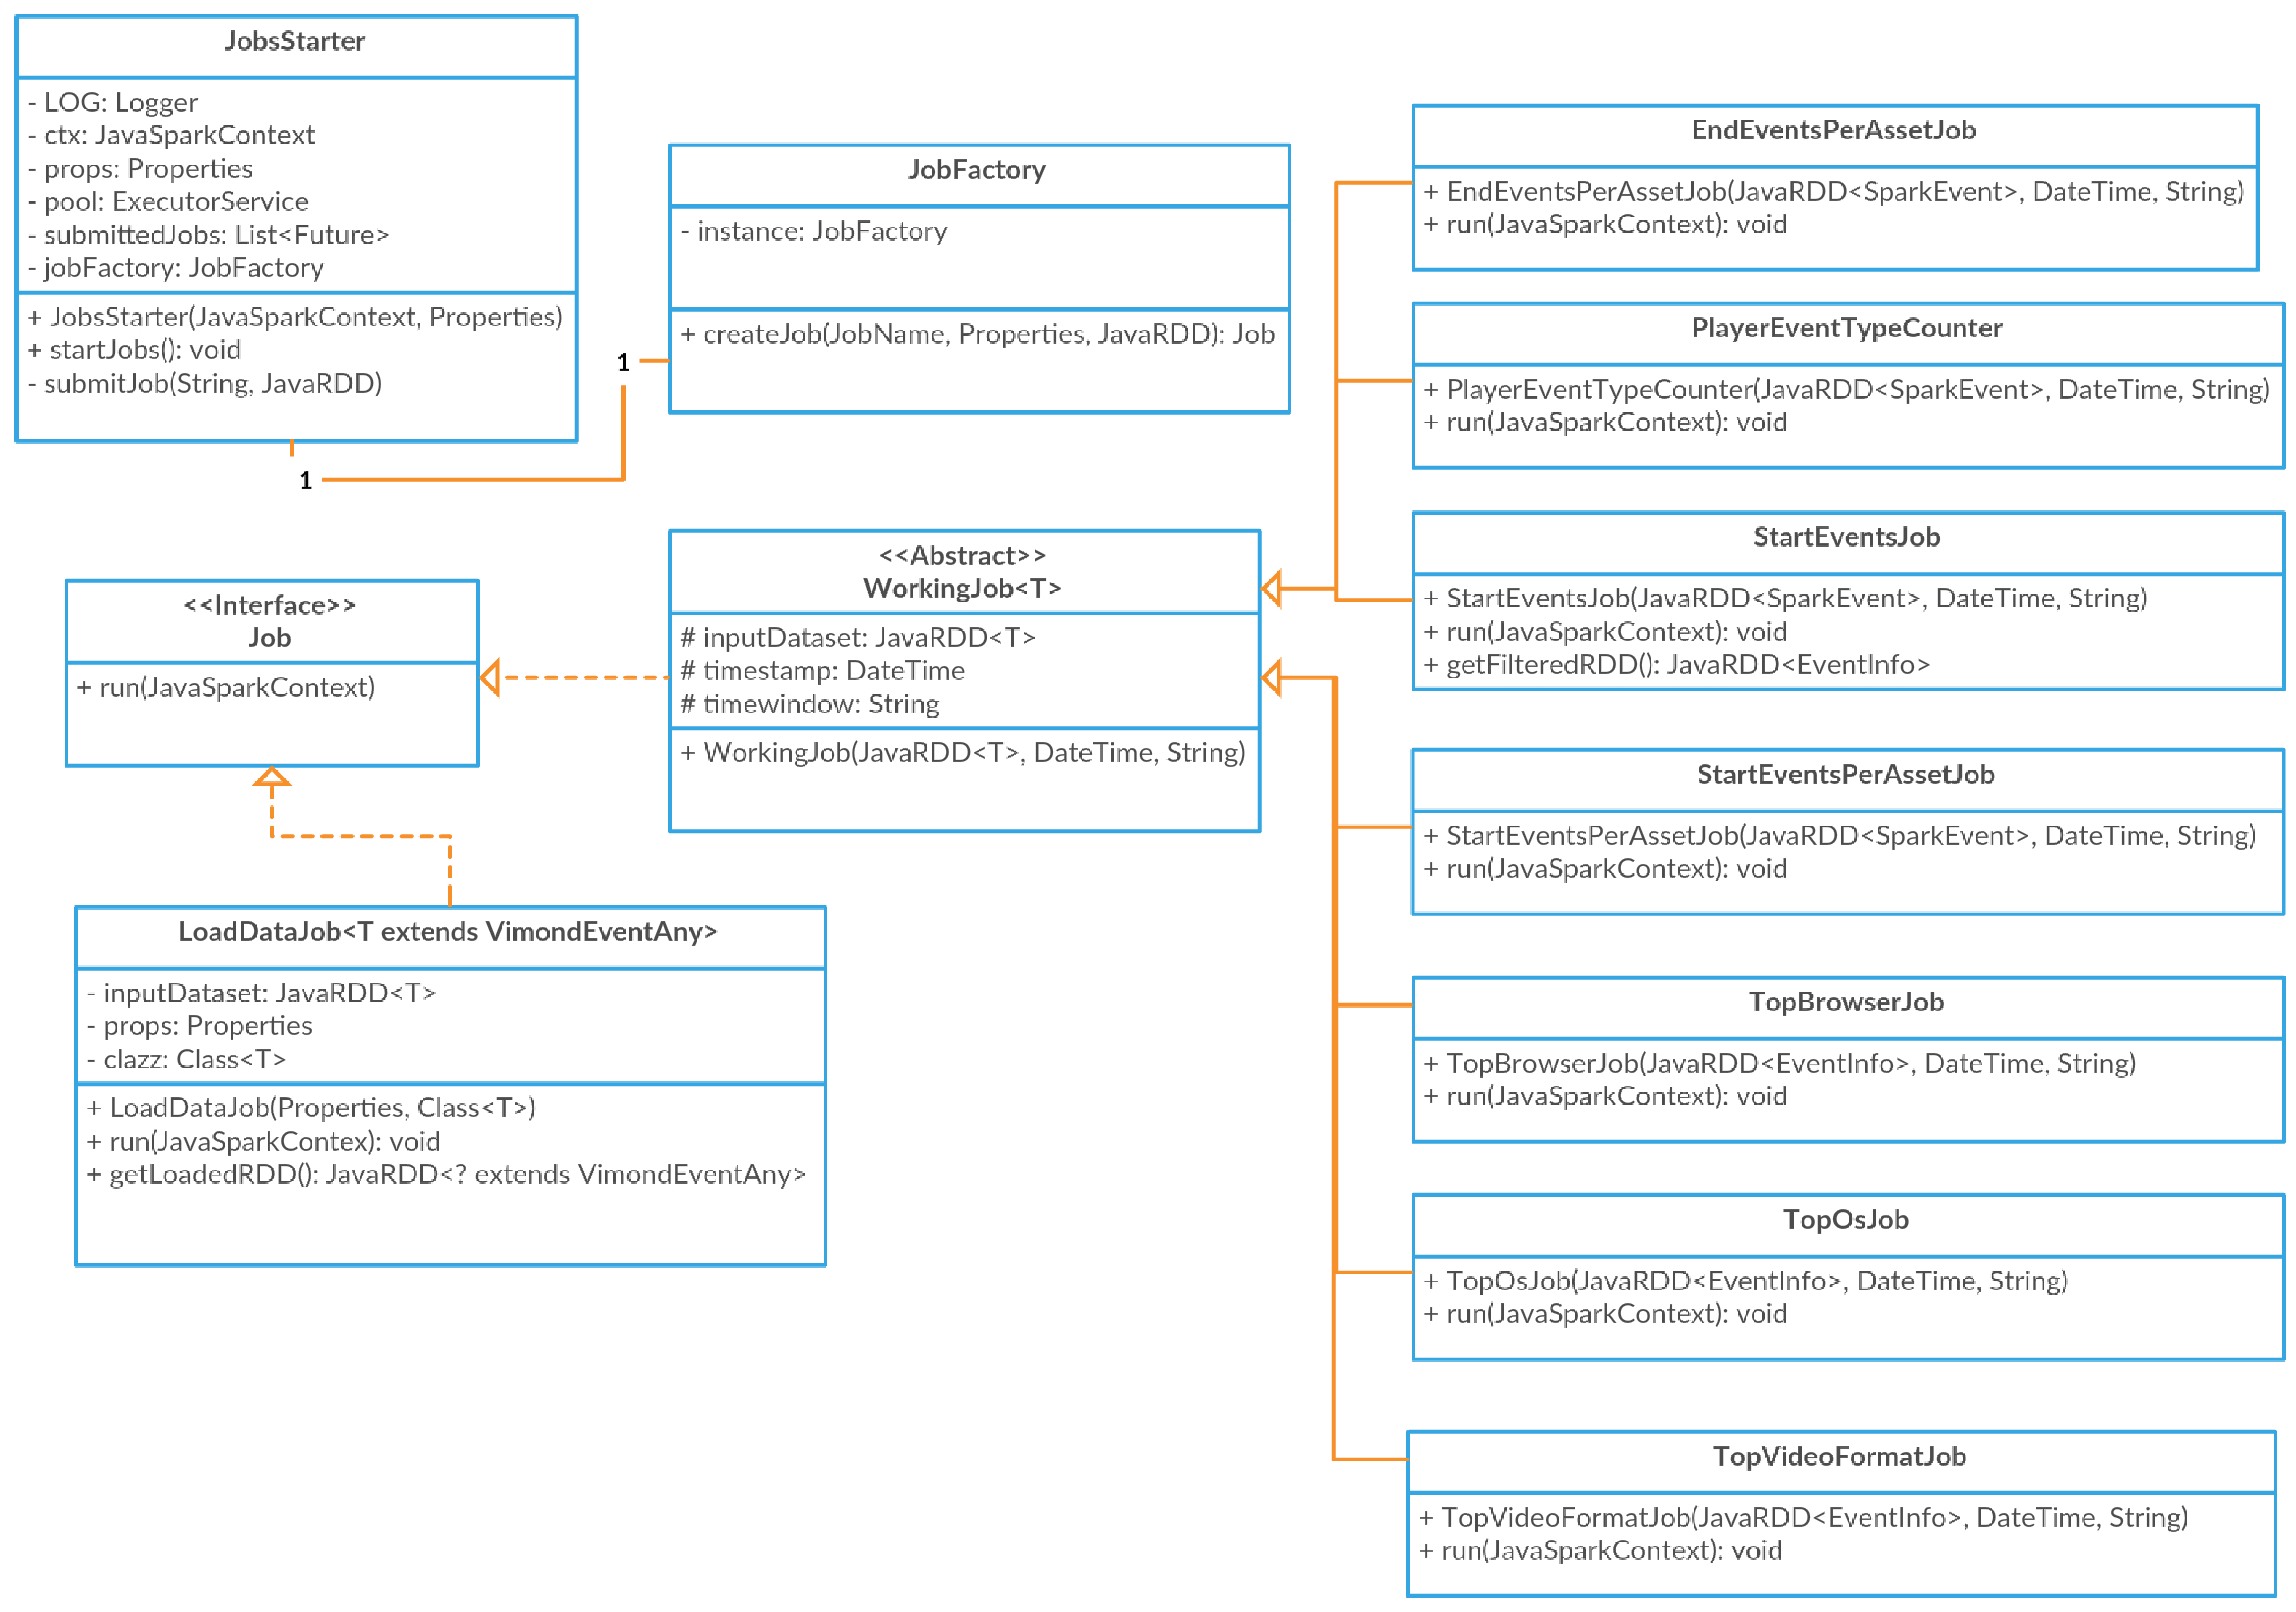
\includegraphics[width=15cm]{imgs/spark-uml.pdf}
\caption[Batch class diagram]{Batch class diagram}
        \label{sparkUML}
\end{figure}

Figure \ref{sparkUML} shows a class diagramm for the most important classes involved in the aggregation process. An aggregation action has been mapped into a Java object implementing the \textit{Job} interface. In addition, for the processes using an input dataset, it has been defined an abstract class named \textit{WorkingJob}. Finally, jobs are started through a \textit{JobStarter} object which uses a factory pattern for jobs creation.

The last step of the batch pipeline is the deletion of the realtime data after the completion of a batch aggregation process over a timewindow of data. This is simply obtained by quering the the serving layer for the data contained in the current time interval and then delete the corresponding results. The serving layer implemented with elasticsearch does not support SQL-like delete operations as \textit{DELETE from table WHERE condition}, but it requires the \textit{id} of the document to be deleted. This process is done in batches in order to improve the throughput of the operations as it would be network expensive sending a delete request for each document. The overall process goes under the name of \textit{delete-by-query}.

\section{Real time layer}

\begin{figure}[h]
       \makebox[\textwidth][c]
       {
        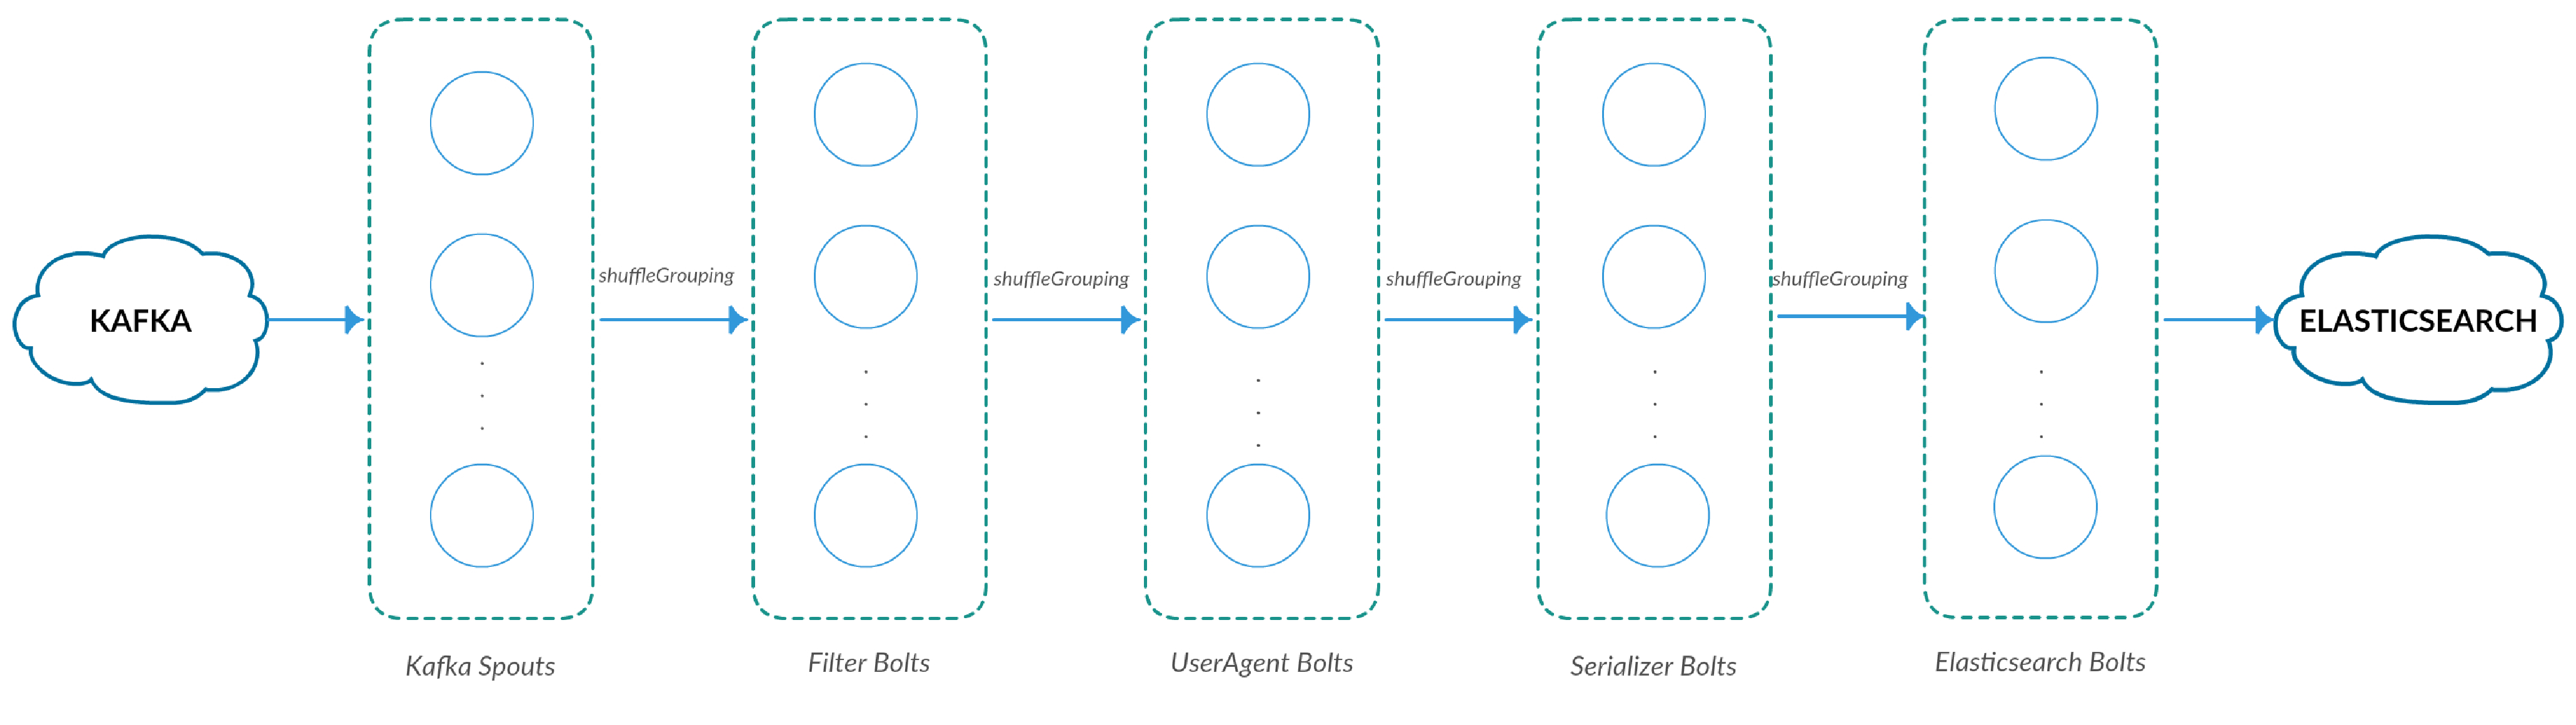
\includegraphics[width=17cm]{imgs/stormTopology}
        }
\caption[Storm real-time topology]{Storm real-time topology}
        \label{stormTopology}
\end{figure}

\section{Serving layer}
The serving layer has been implented using Elasticsearch. As stated in chapter \ref{chap:chapter2}, Elasticsearch provides storage space for documents and a \textit{Lucene} search engine for querying them. Moreover it works with documents in JSON format, making easy to query and aggretate them according to a specific field inside them.

Mapping.\\Query\\Kibana

\section{Tuning}
\subsection{RealTime}
Serialization with kryo rather than objectmapper. show benchmark analysis  on serialization libraries


\appendix
\chapter*{Appendix A\\ Framework configurations}
\label{appendix}
In this section we are going to report the followed procedures for installing and setting up the frameworks used in this thesis work.
\section{Apache Oozie}

The version used for this project is the 4.2.0 (stable version - June 2015). The procedure for the installation is not trivial, as you need to build a working distro from source code.
Prerequisites:
\begin{itemize}
\item Java 1.6+
\item Apache Hadoop
\item Apache Maven
\item ext-2.2
\end{itemize}
Java 1.8, hadoop 2.7.0 and maven 3.3.3 were used during the installation procedure.\\
It is assumed also that hadoop is running using the default ports setting
\subsection{Installation\protect\footnote{At the time of installation I came across a bug due to a repository out of service. Refer to \cite{bib3} for its solution}}
\begin{lstlisting}[language=sh]
#donwload the tarball from a mirror
cd ~
wget http://apache.uib.no/oozie/4.2.0/oozie-4.2.0.tar.gz 
tar -xvf oozie-4.2.0.tar.gz

#build a distro according to your java version and hadoop version
cd oozie-4.2.0/bin
./mkdistro -DtargetJavaVersion=1.8 -P hadoop-2 -Dhadoop.version=2.7.0 

#configure the distro
cd distro/target/oozie-4.2.0
mkdir libext
mv /path/to/ext-2.2.zip libext
bin/oozie-setup.sh sharelib create -fs hdfs://localhost:9000
bin/oozie-setup.sh prepare-war
bin/ooziedb.sh create -sqlfile oozie.sql -run
bin/oozied.sh start
\end{lstlisting}

In order to set up the integration with hadoop, the following properties need to be defined:

\begin{lstlisting}[language=XML]
<!-- oozie-site.xml -->
<property>
    <name>oozie.service.HadoopAccessorService.hadoop.configurations</name>
	<value>*=/path/to/hadoop-2.7.0/etc/hadoop</value>
</property>
<property>
     <name>oozie.service.WorkflowAppService.system.libpath</name>
     <value>hdfs:///user/${user.name}/share/lib</value>
</property>

<!-- hadoop core-site.xml -->
<property>
      <name>hadoop.proxyuser.myhadoopusername.hosts</name>
      <value>*</value>
</property>
<property>
      <name>hadoop.proxyuser.myhadoopusername.groups</name>es
      <value>*</value>
</property>

\end{lstlisting}

Once oozie is started, is it possible to control the job executions via web interface at $localhost:11000$


 





% ELENCO DELLE FIGURE (OPZIONALE)
\addcontentsline{toc}{chapter}{List of Figures}
\listoffigures


% BIBLIOGRAFIA
\addcontentsline{toc}{chapter}{Bibliography}
\begin{thebibliography}{9}
        \bibitem{bib1}B. Urgaonkar ,
G. Pacifici , P. Shenoy , M. Spreitzer , A. Tantawi,
            \emph{``“An analytical model for multi­tier internet services and its applications''}
        \bibitem{bib2} Giuseppe Iazeolla, 
            \emph{``Impianti Reti Sistemi Informatici''},
\end{thebibliography}
\end{document}
